\chapter{Hình ảnh và bảng trích từ bài báo gốc}
\label{app:original-paper}
\setcounter{figure}{0}
\renewcommand{\thefigure}{D.\arabic{figure}}
\setcounter{table}{0}
\renewcommand{\thetable}{D.\arabic{table}}

\noindent Phụ lục này lưu các hình và bảng gốc được trích từ bài báo của Eskandari et al. (2024), \emph{Applied Energy}, 366, 123314 [1]. Các ảnh được trích từ PDF bài báo, giữ nguyên nội dung biểu đồ, chú giải và dữ liệu hiển thị; không dựng lại bằng dữ liệu KAG và không chỉnh sửa giá trị. Mục đích là cung cấp nguồn trực quan để đối chiếu các mô tả trong Chương 5. Số trang ghi trong caption là số trang của bài báo gốc.

\section{Các hình mô tả bối cảnh và phương pháp}

\begin{figure}[p]
\centering
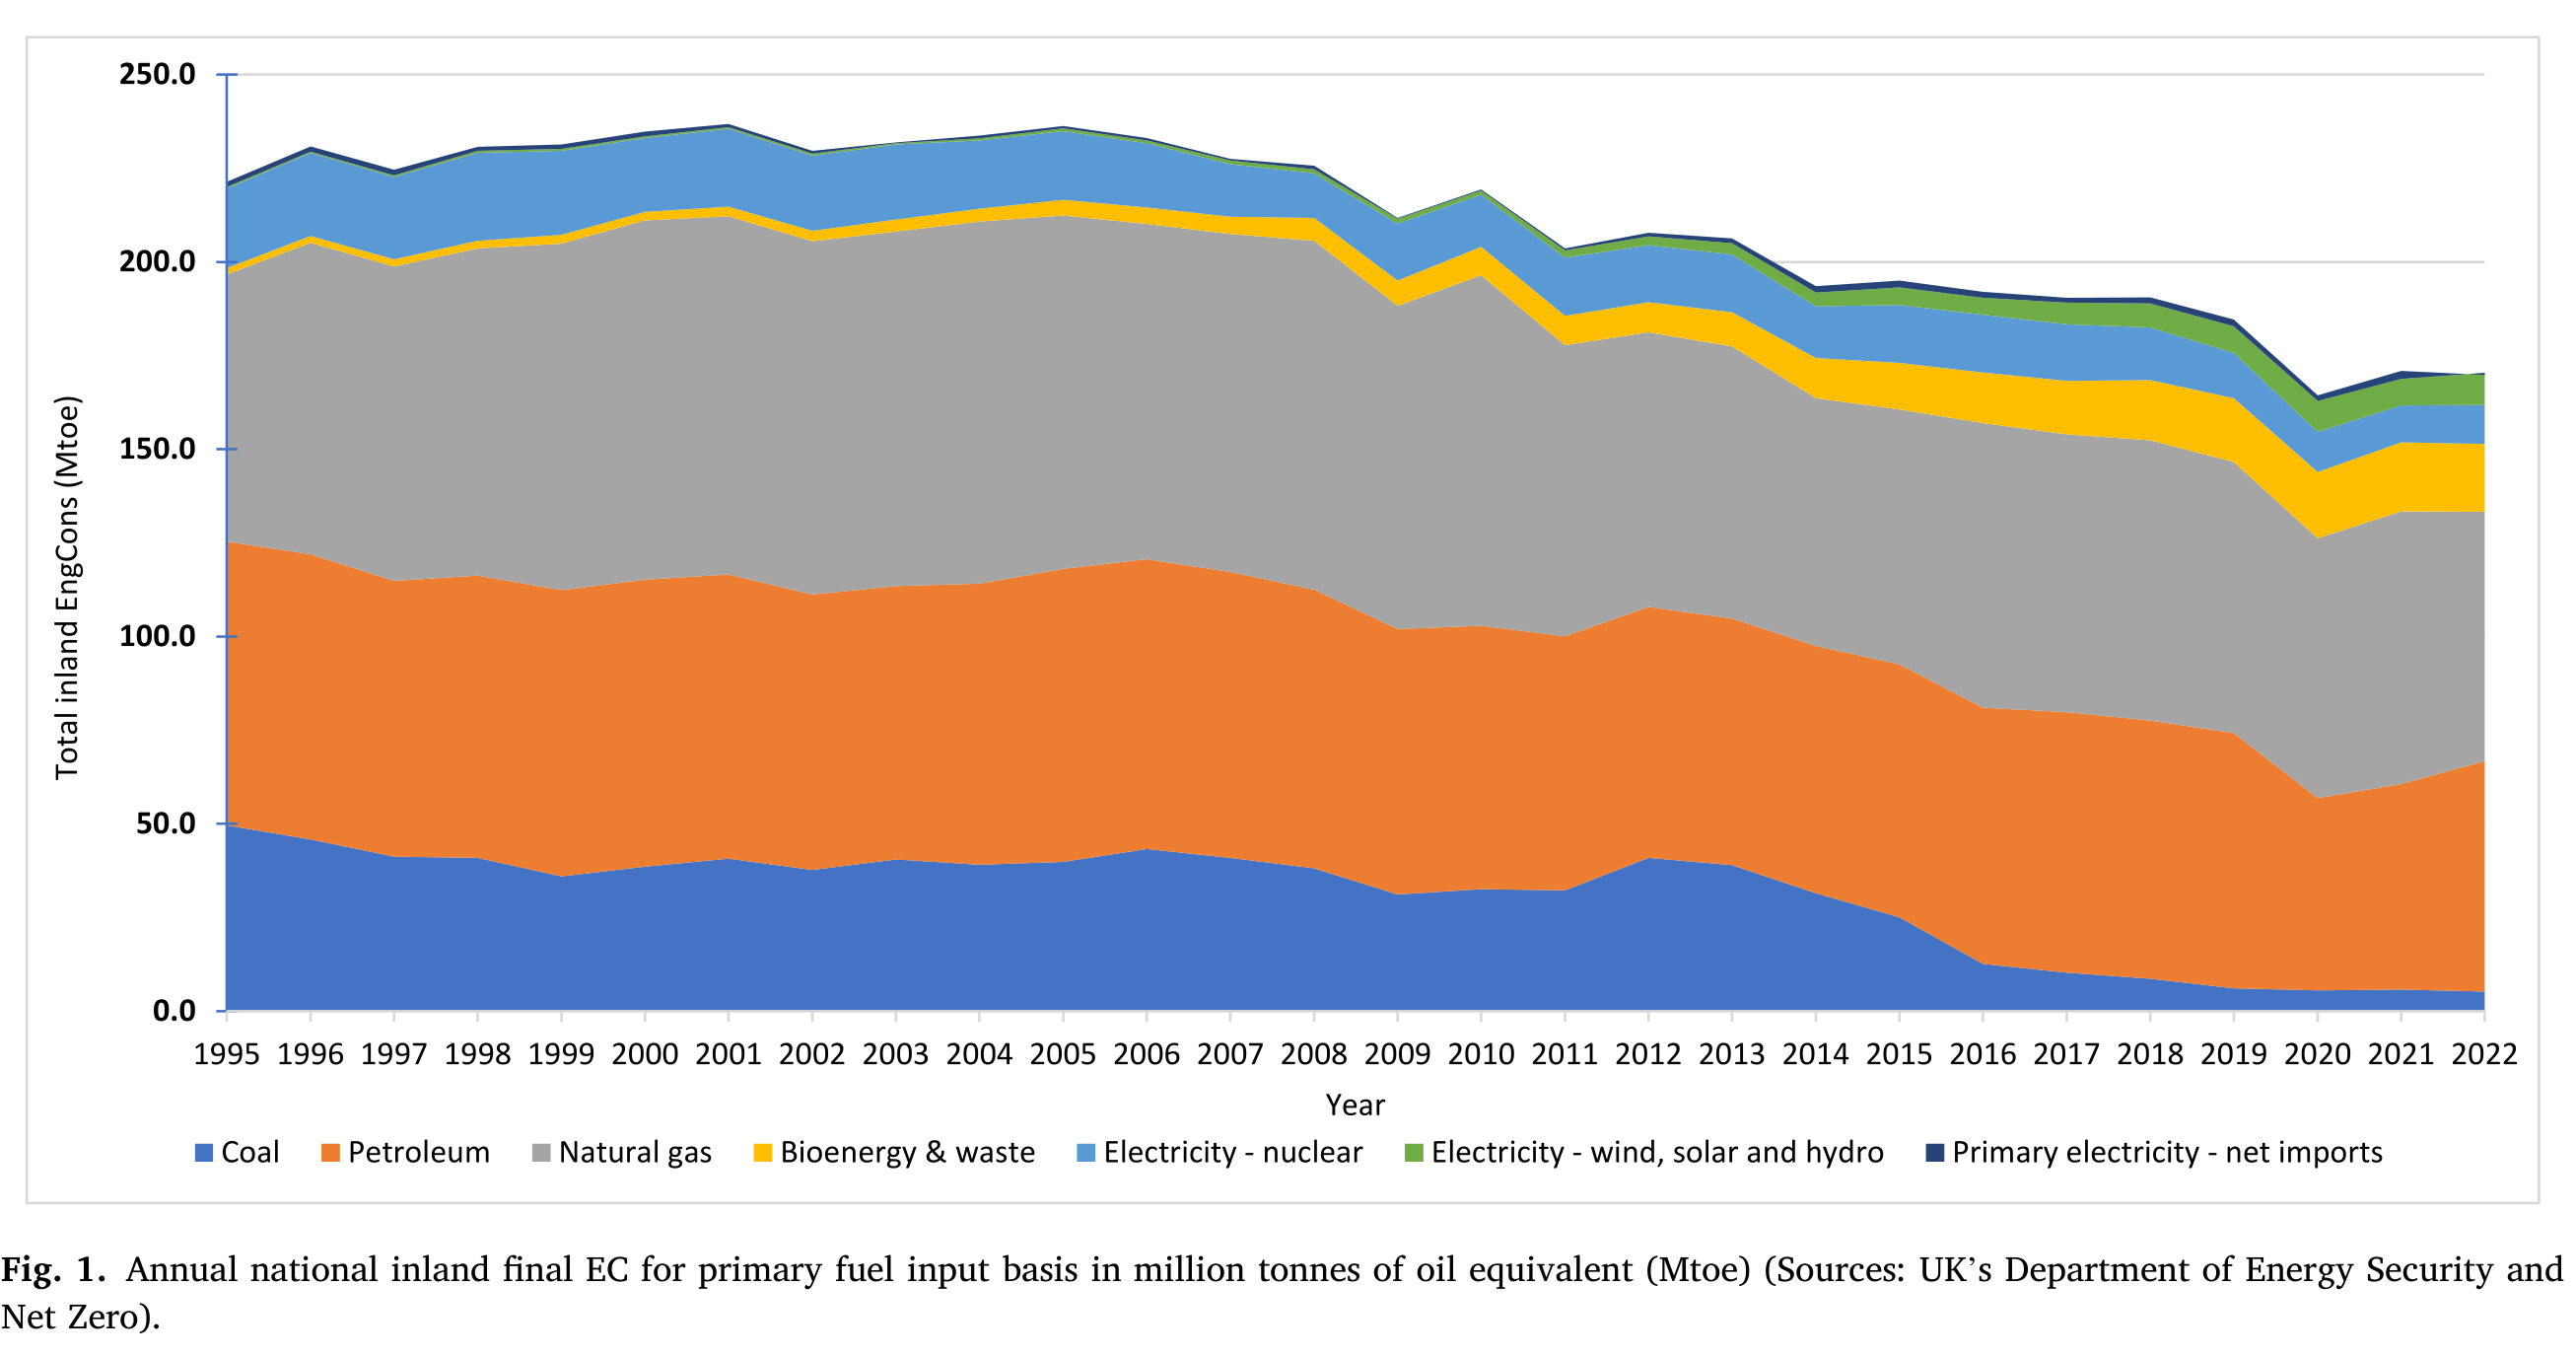
\includegraphics[width=0.96\textwidth,height=0.70\textheight,keepaspectratio]{figures/paper_original/fig01_annual_energy_mix.png}
\caption{Hình 1 trong bài báo gốc: cơ cấu tiêu thụ năng lượng nội địa cuối cùng theo nguồn năng lượng tại Vương quốc Anh. Nguồn: Eskandari et al. [1], tr. 2.}
\label{fig:orig-01}
\end{figure}

\begin{figure}[p]
\centering
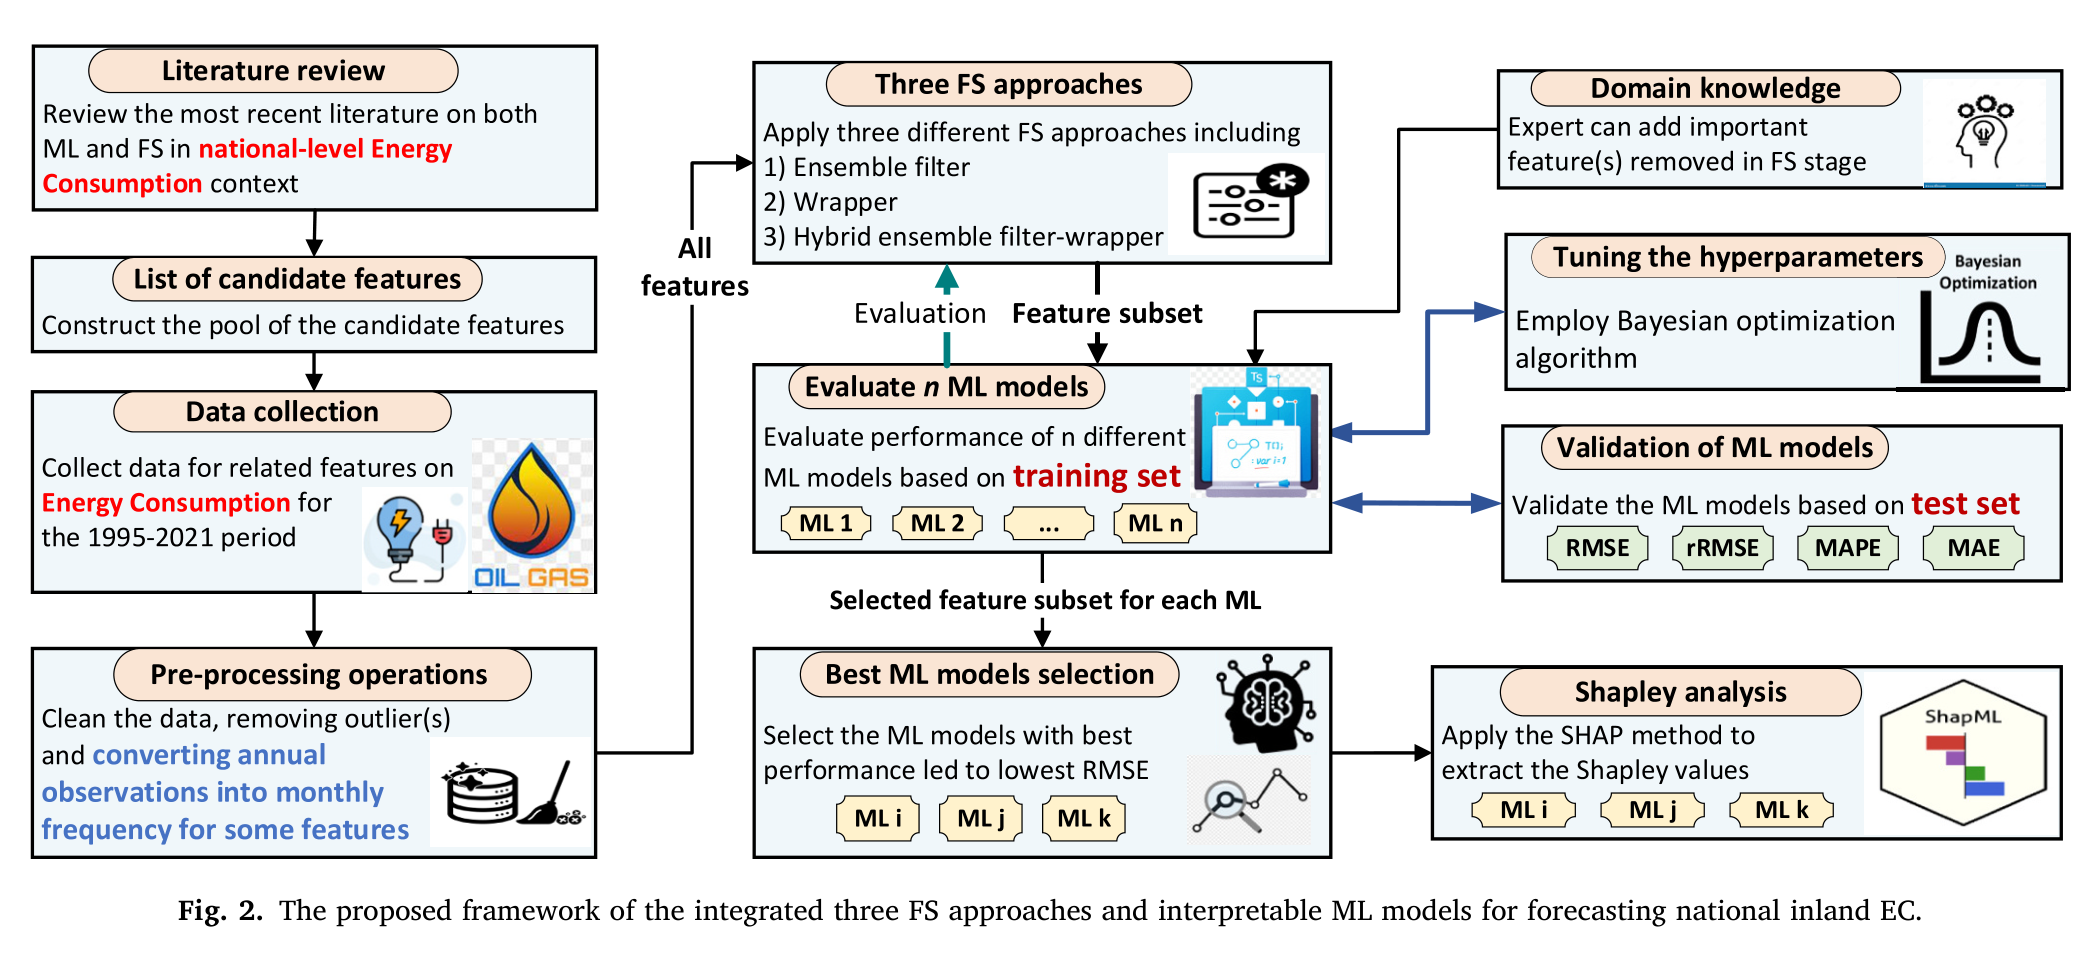
\includegraphics[width=0.98\textwidth,height=0.66\textheight,keepaspectratio]{figures/paper_original/fig02_framework.png}
\caption{Hình 2 trong bài báo gốc: framework tích hợp ba chiến lược Feature Selection, các mô hình ML, Bayesian Optimization, validation và SHAP. Nguồn: [1], tr. 3.}
\label{fig:orig-02}
\end{figure}

\begin{figure}[p]
\centering
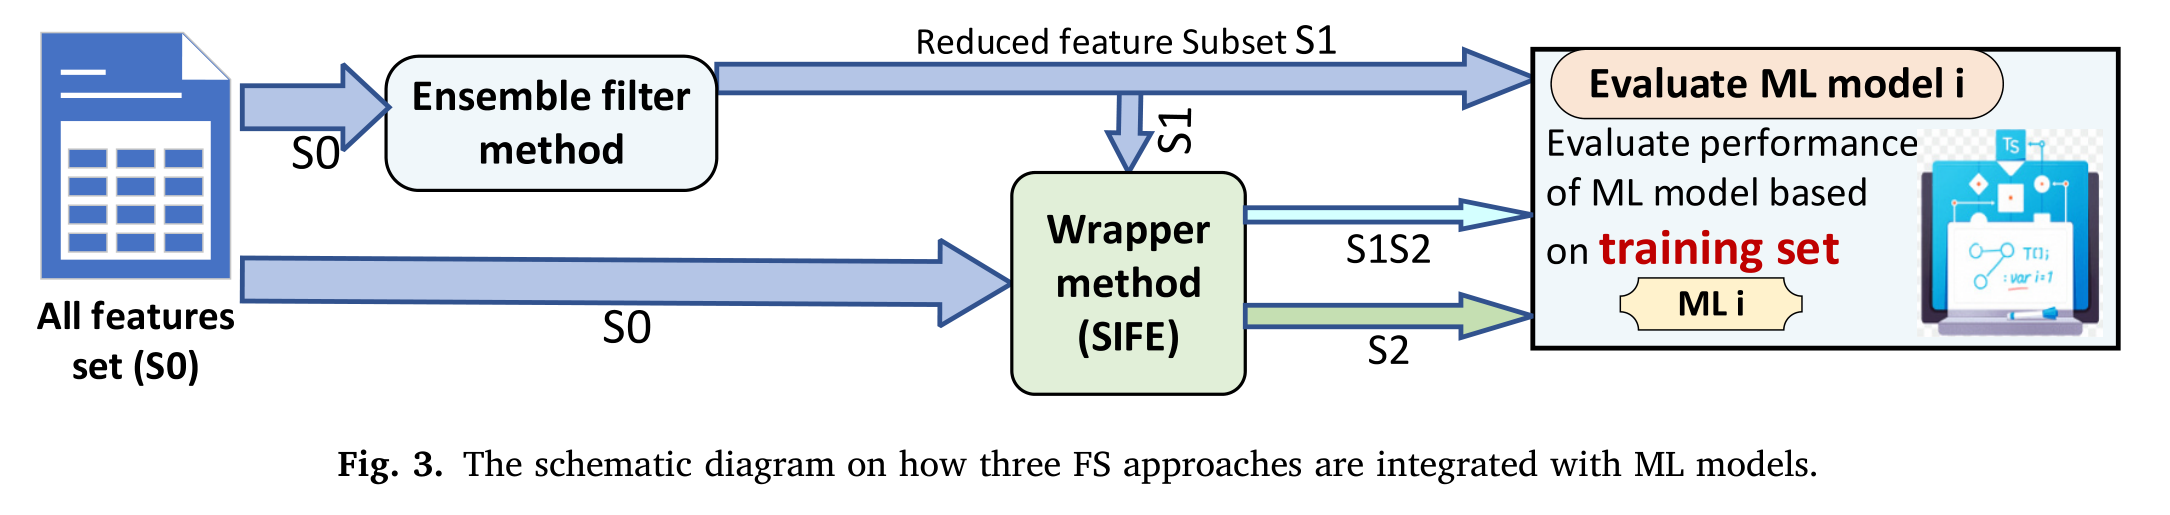
\includegraphics[width=0.98\textwidth,height=0.60\textheight,keepaspectratio]{figures/paper_original/fig03_three_fs_workflow.png}
\caption{Hình 3 trong bài báo gốc: sơ đồ tích hợp ba nhánh S1, S2 và S1S2 với các mô hình ML. Nguồn: [1], tr. 6.}
\label{fig:orig-03}
\end{figure}

\begin{figure}[p]
\centering
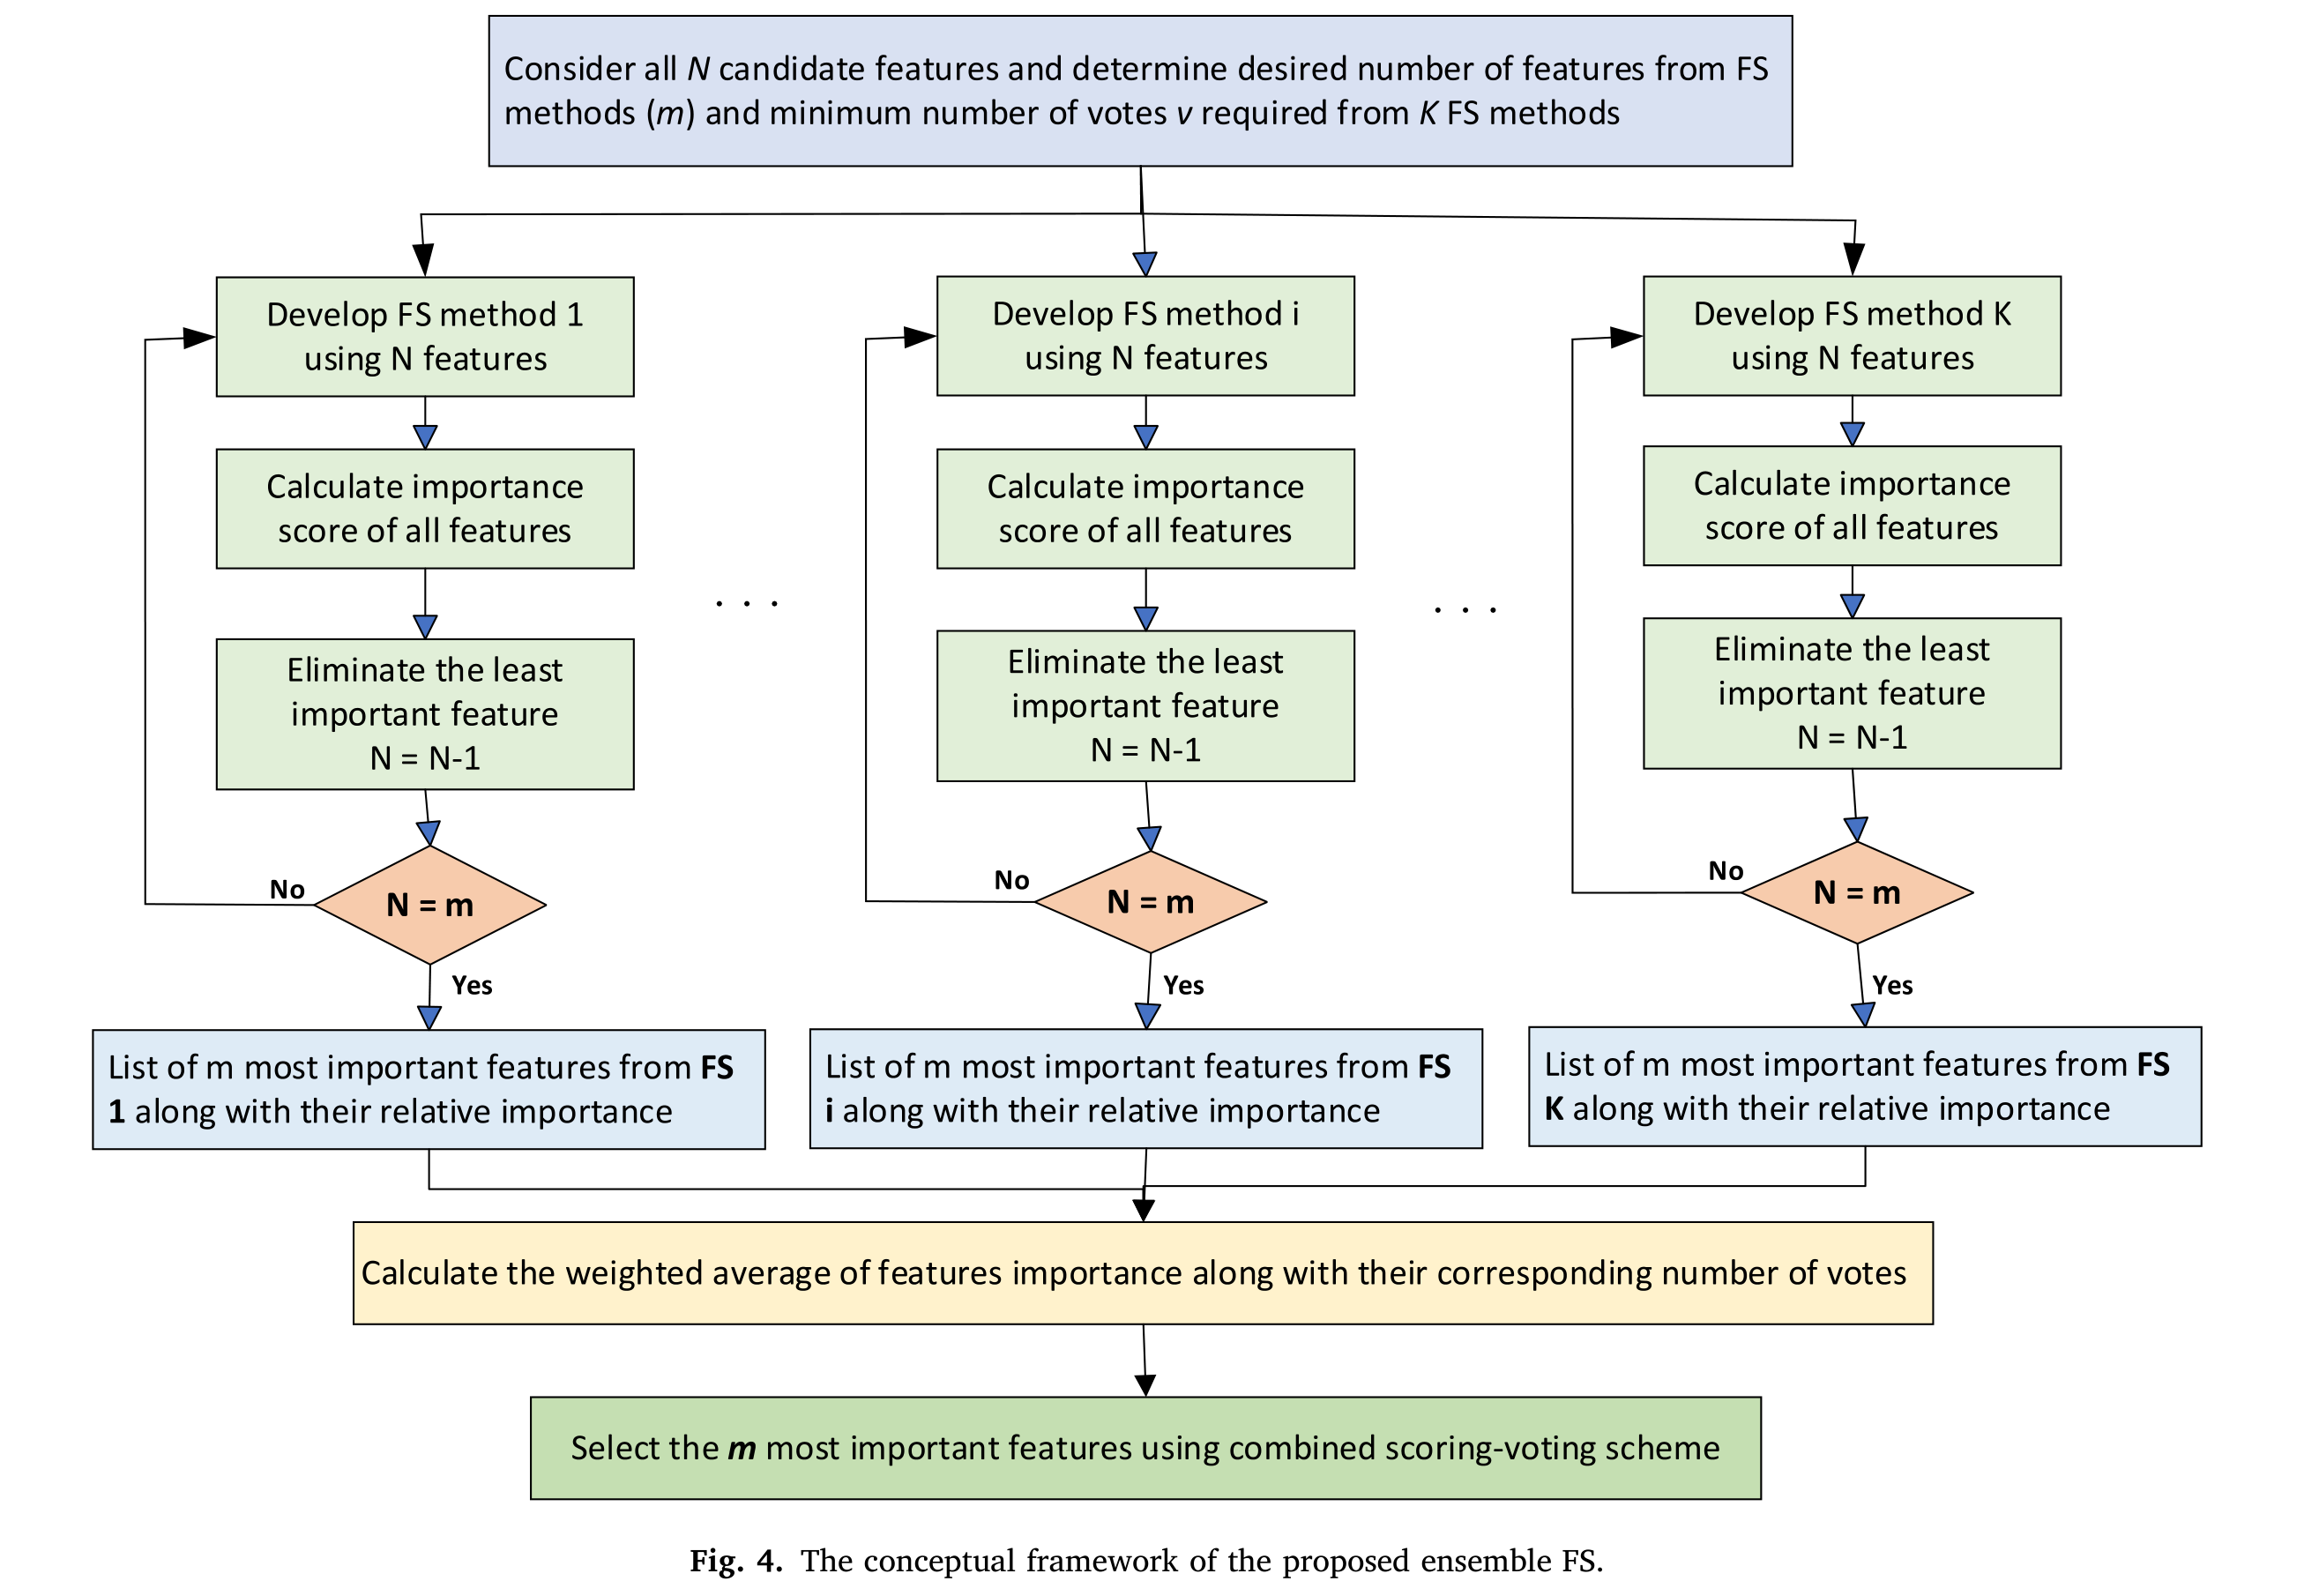
\includegraphics[width=0.98\textwidth,height=0.66\textheight,keepaspectratio]{figures/paper_original/fig04_ensemble_filter.png}
\caption{Hình 4 trong bài báo gốc: quy trình Ensemble Filter với loại dần đặc trưng, tổng hợp importance và voting. Nguồn: [1], tr. 7.}
\label{fig:orig-04}
\end{figure}

\section{Các hình mô tả dữ liệu và phân tích đặc trưng}

\begin{figure}[p]
\centering
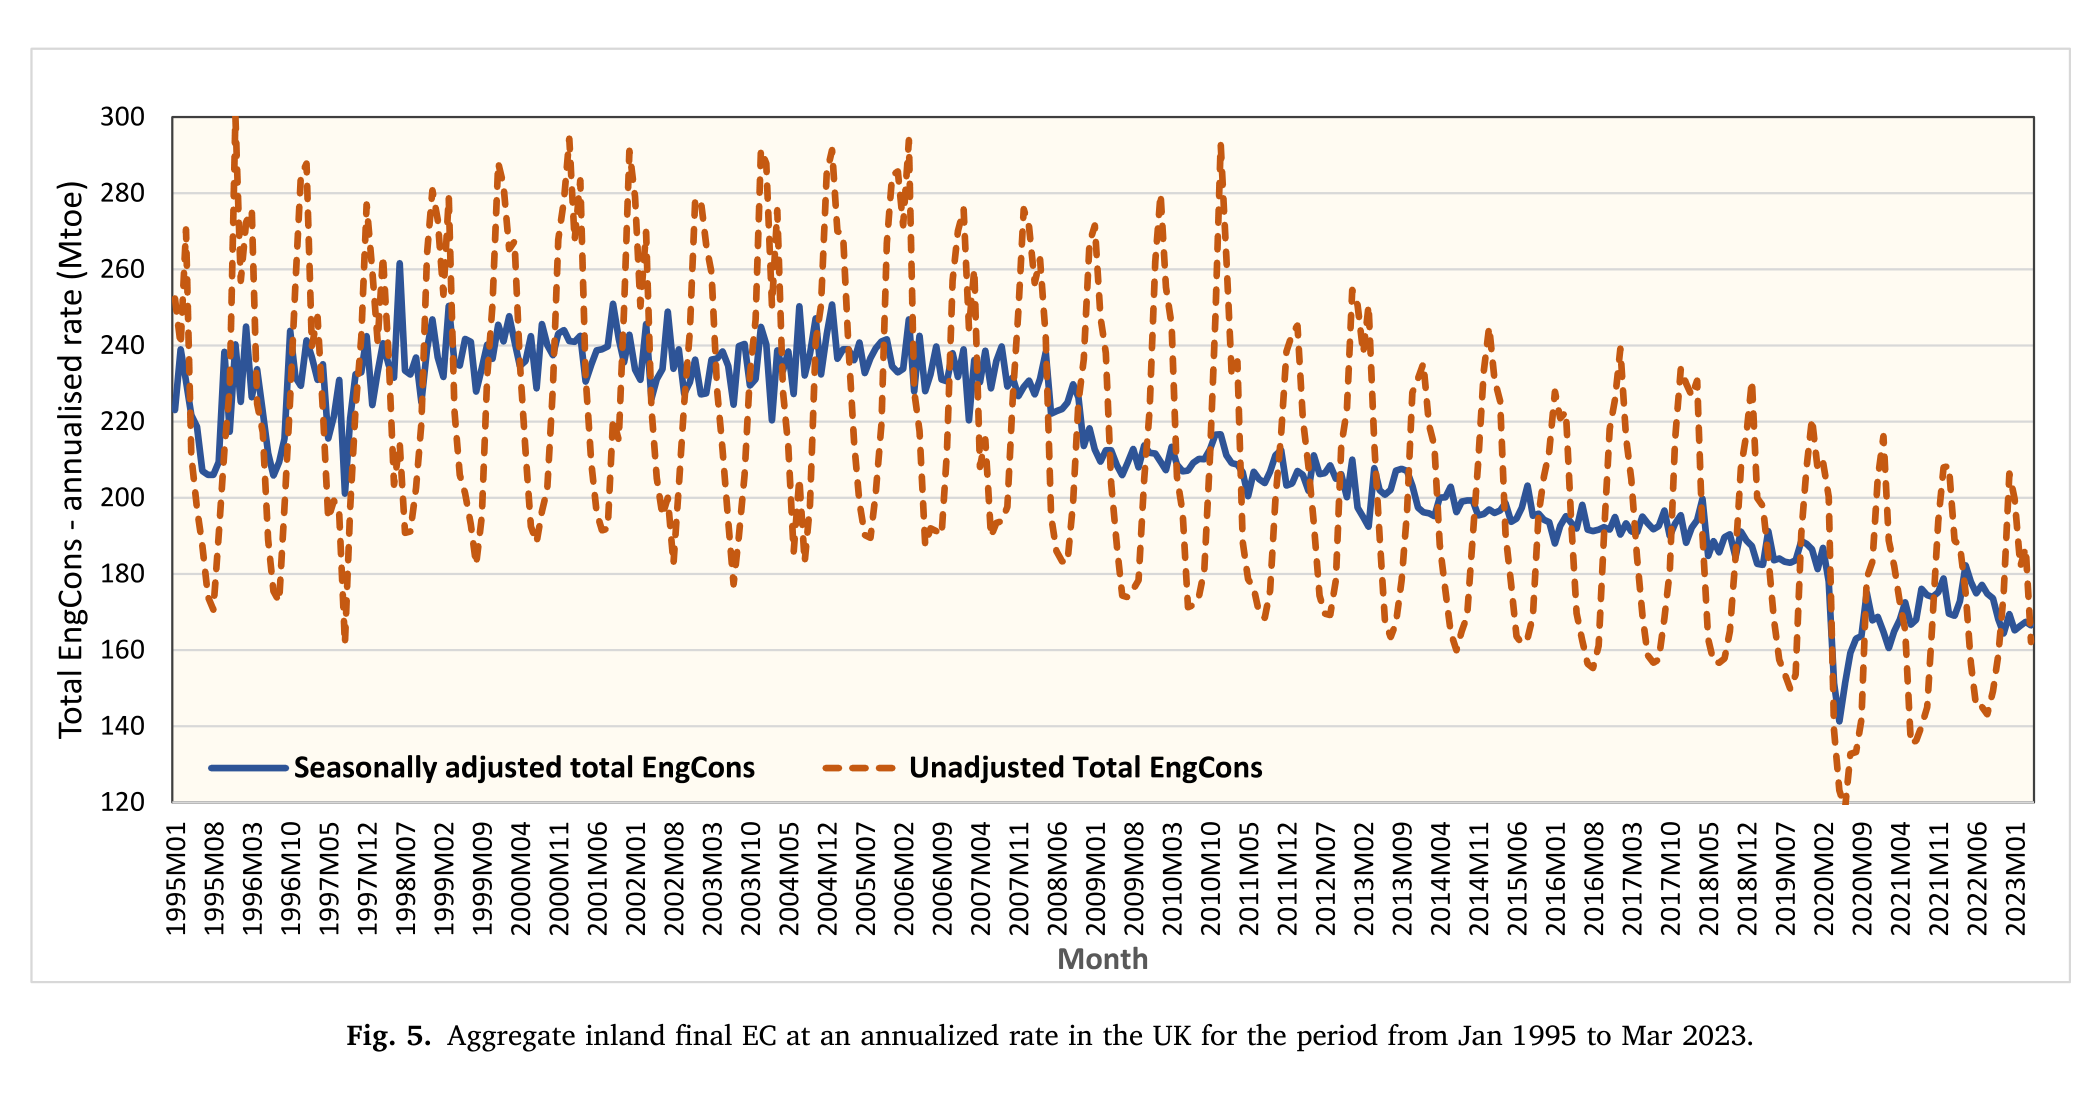
\includegraphics[width=0.98\textwidth,height=0.65\textheight,keepaspectratio]{figures/paper_original/fig05_uk_monthly_ec.png}
\caption{Hình 5 trong bài báo gốc: diễn biến tổng tiêu thụ năng lượng nội địa cuối cùng theo tháng tại Vương quốc Anh. Nguồn: [1], tr. 10.}
\label{fig:orig-05}
\end{figure}

\begin{figure}[p]
\centering
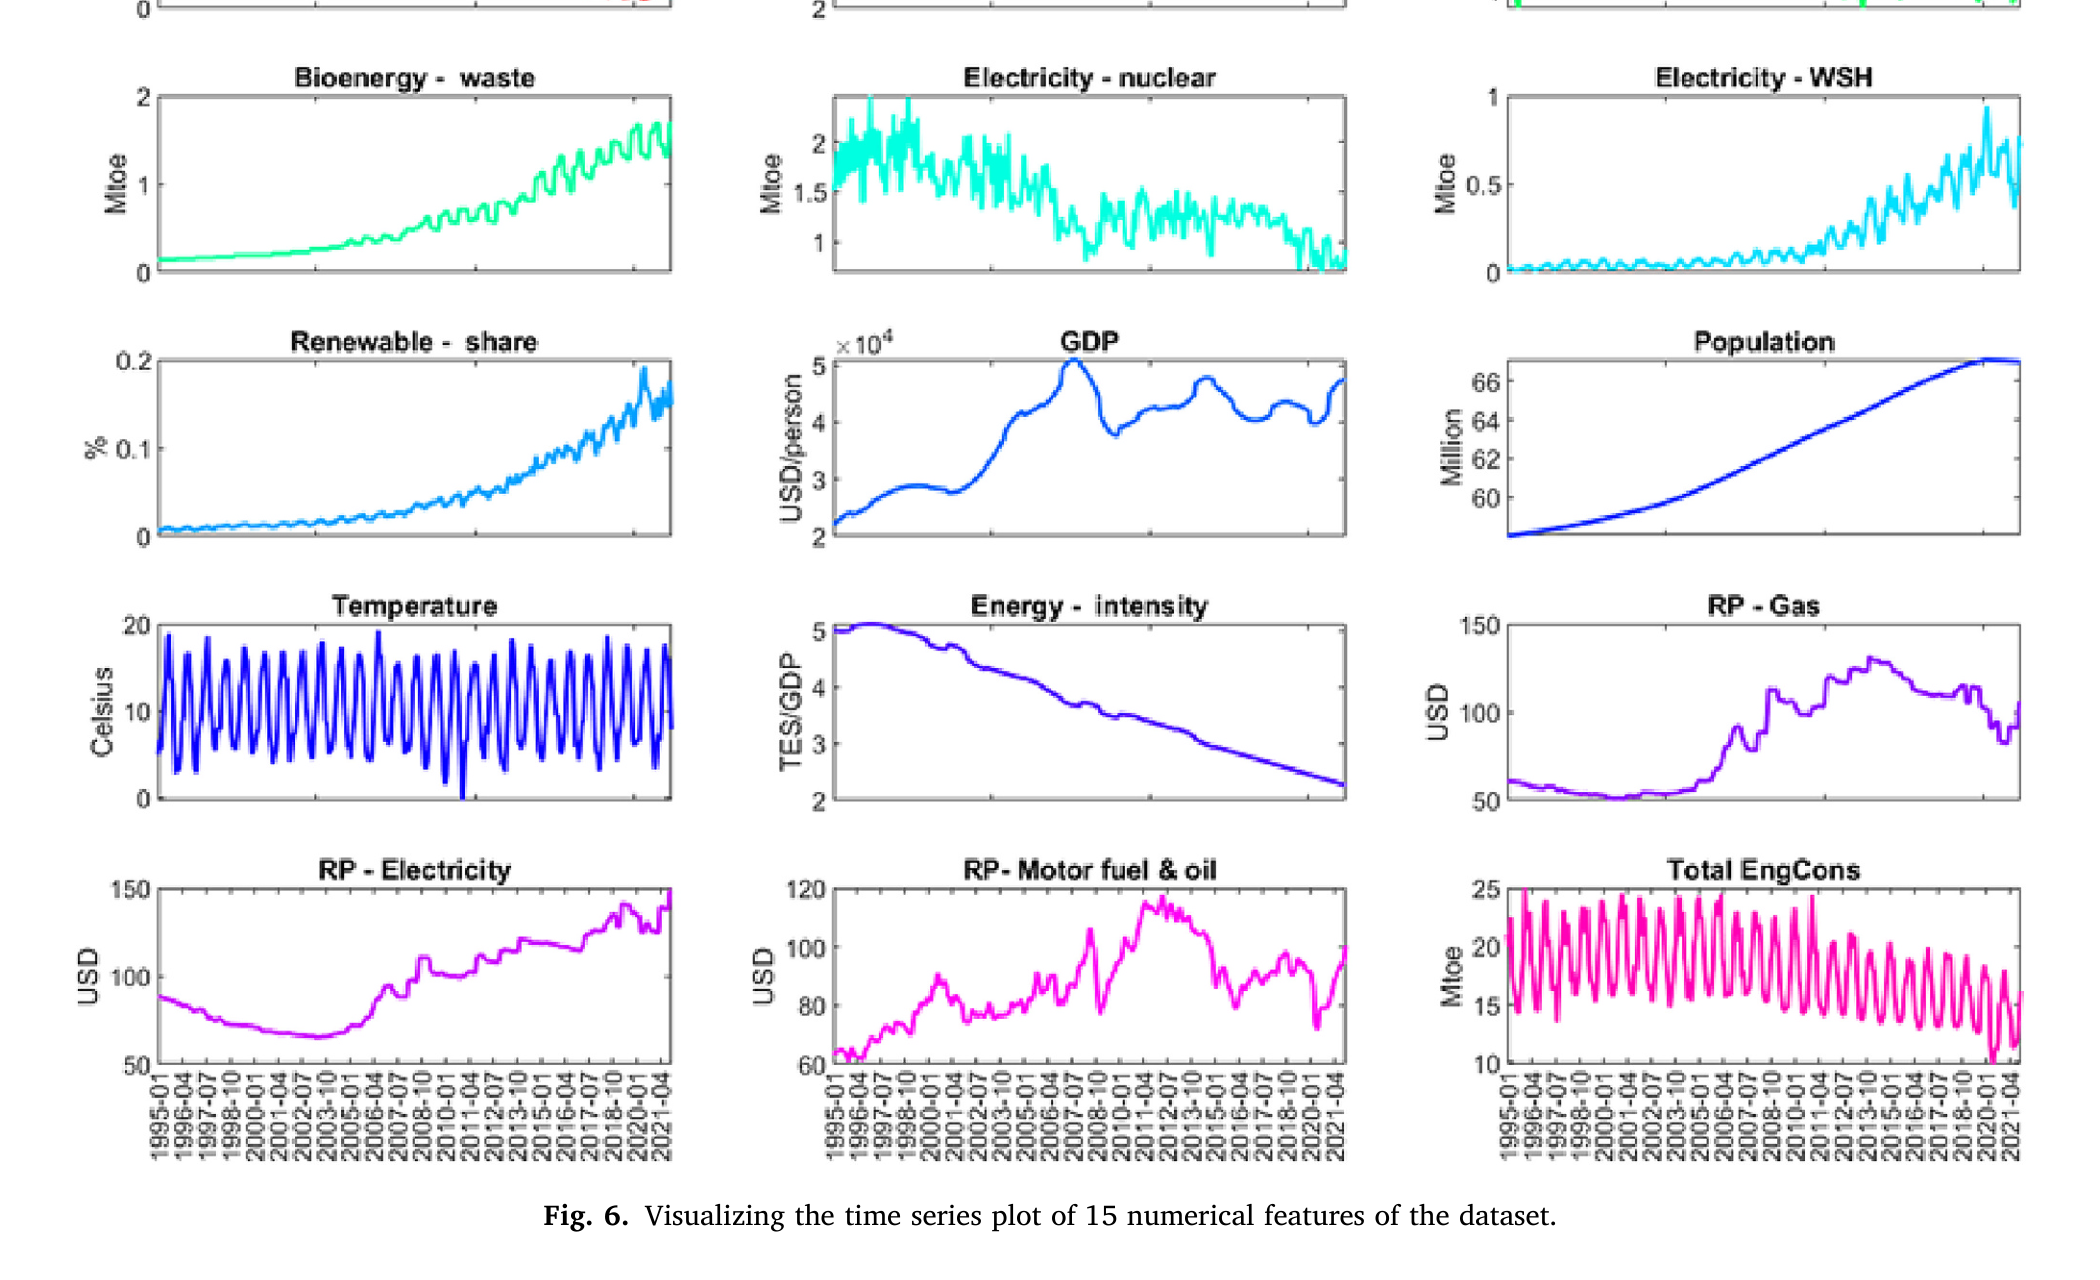
\includegraphics[width=0.98\textwidth,height=0.70\textheight,keepaspectratio]{figures/paper_original/fig06_original_feature_series.png}
\caption{Hình 6 trong bài báo gốc: chuỗi thời gian của 15 biến số chính được sử dụng trong nghiên cứu. Nguồn: [1], tr. 11.}
\label{fig:orig-06}
\end{figure}

\begin{figure}[p]
\centering
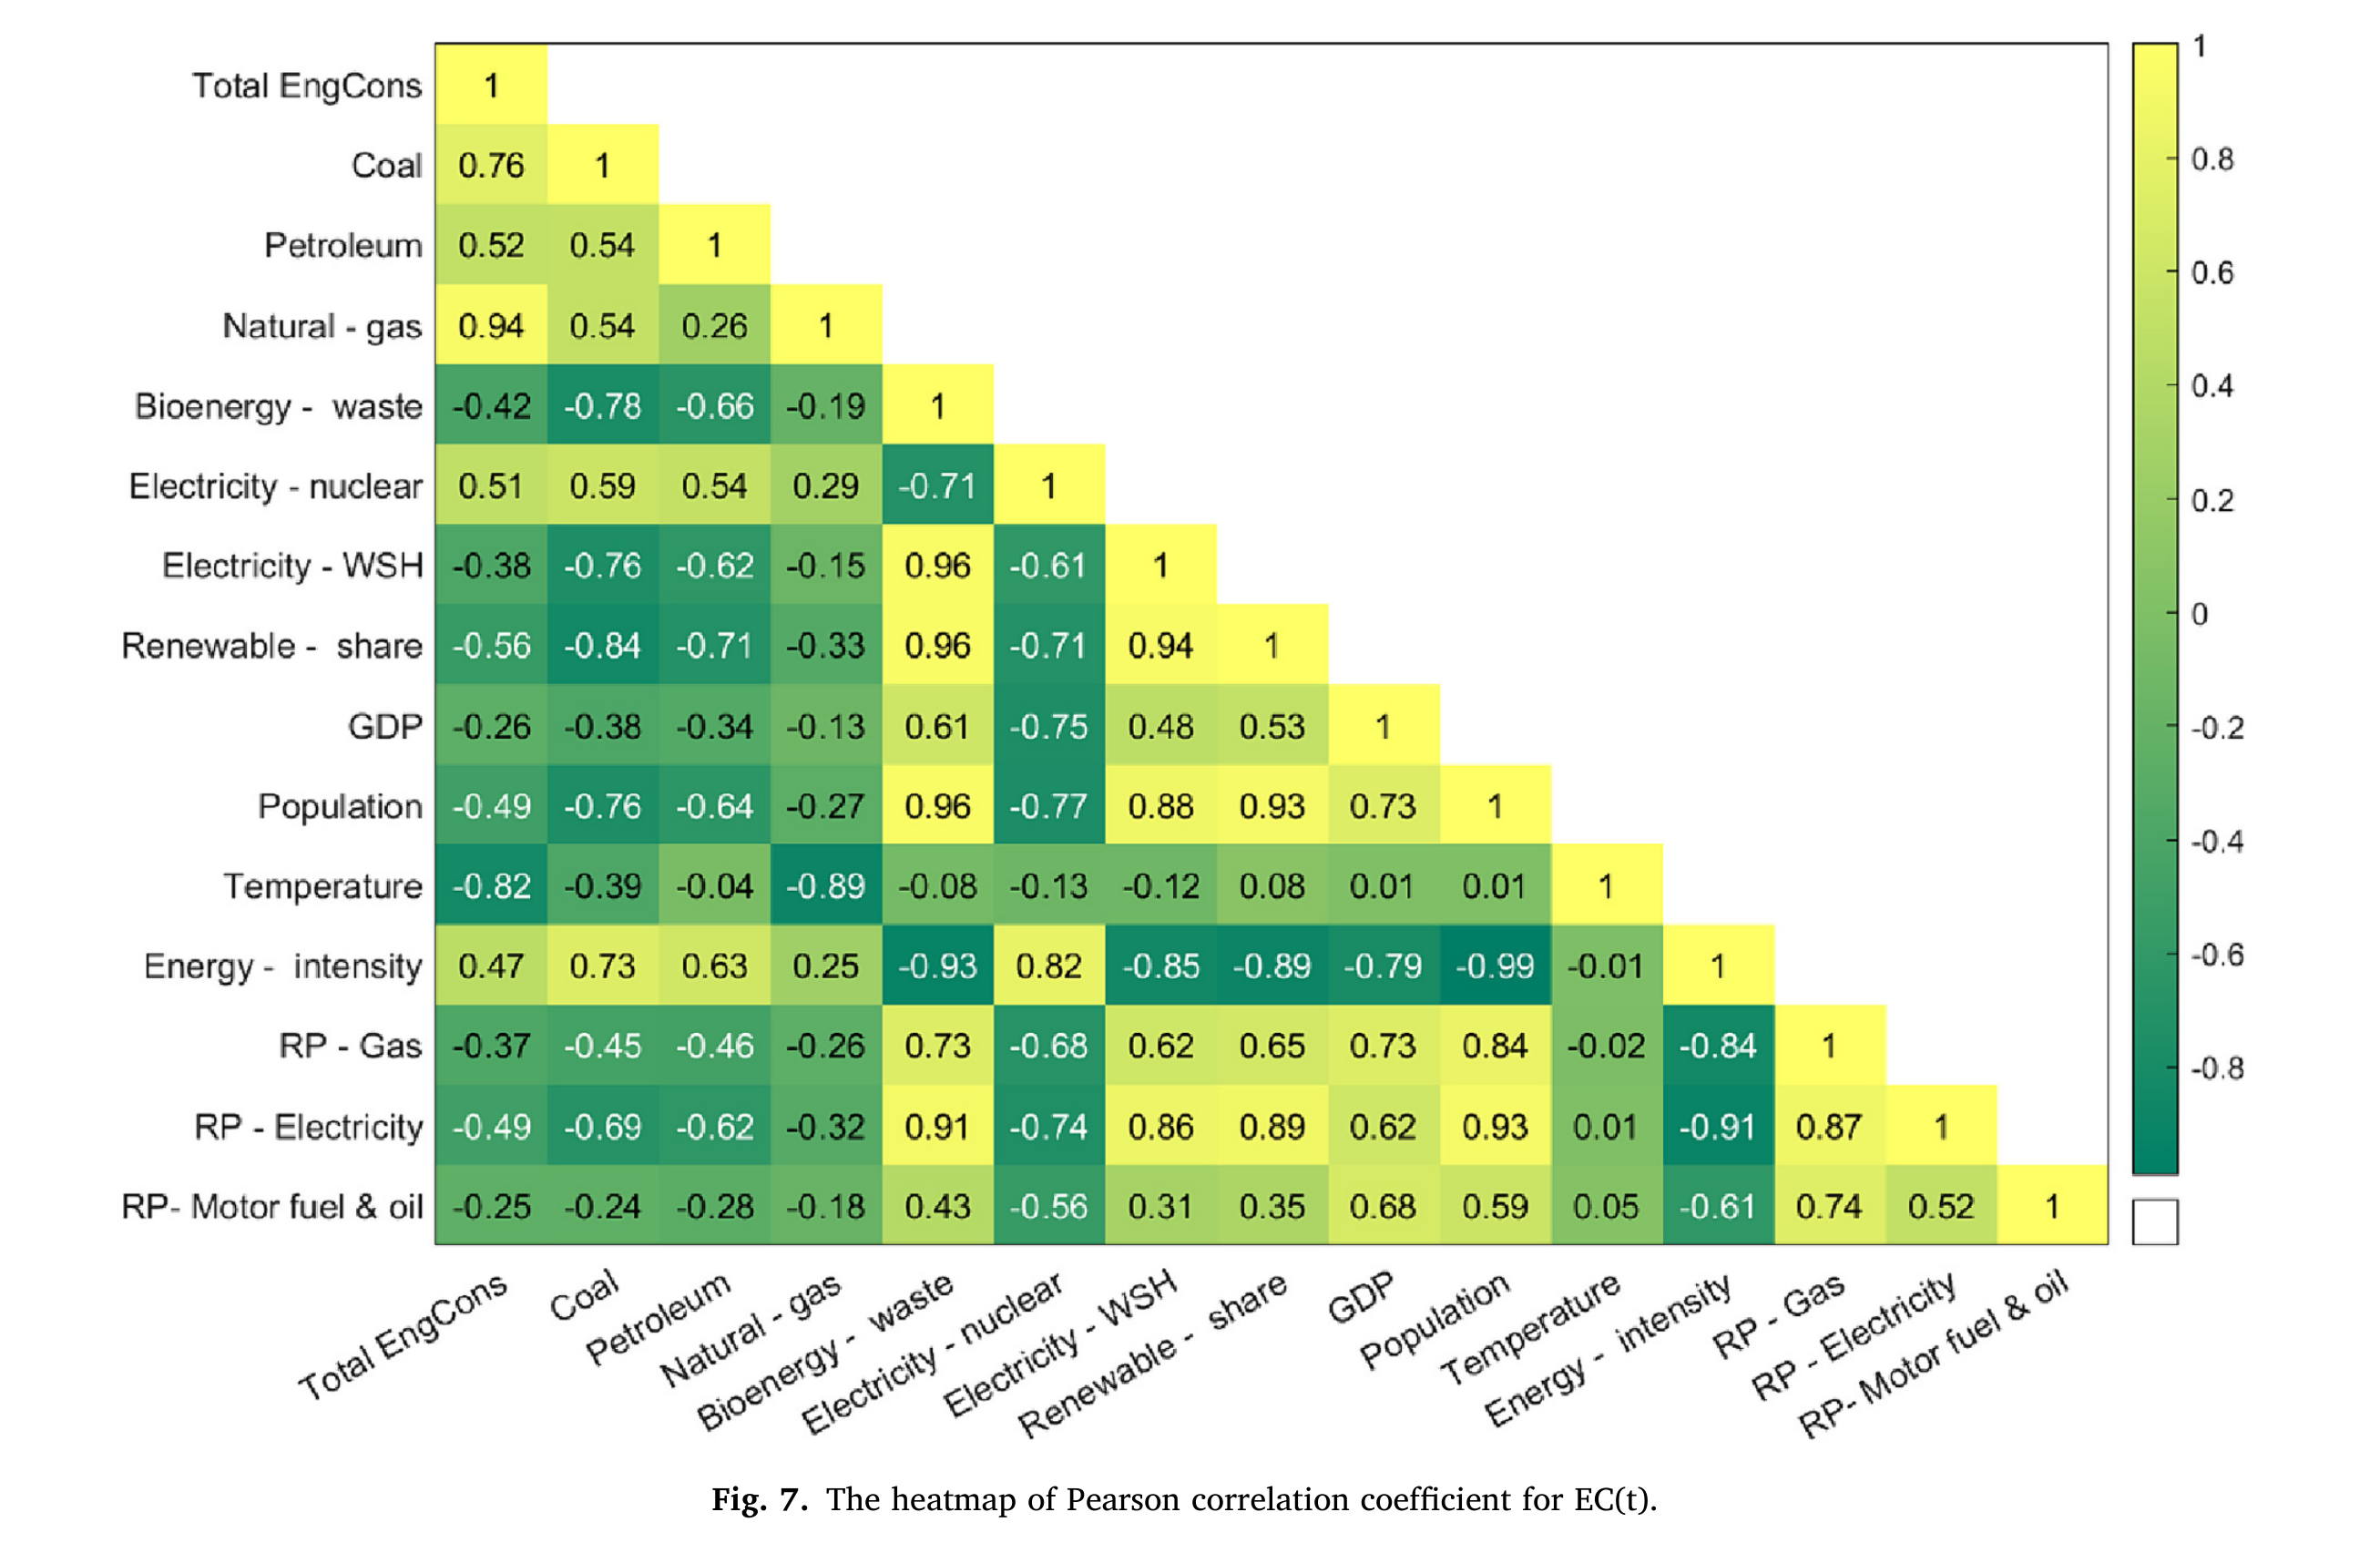
\includegraphics[width=0.98\textwidth,height=0.68\textheight,keepaspectratio]{figures/paper_original/fig07_pearson_heatmap.png}
\caption{Hình 7 trong bài báo gốc: heatmap hệ số tương quan Pearson giữa các biến tiêu thụ năng lượng và biến giải thích. Nguồn: [1], tr. 13.}
\label{fig:orig-07}
\end{figure}

\section{Các hình kết quả dự báo}

\begin{figure}[p]
\centering
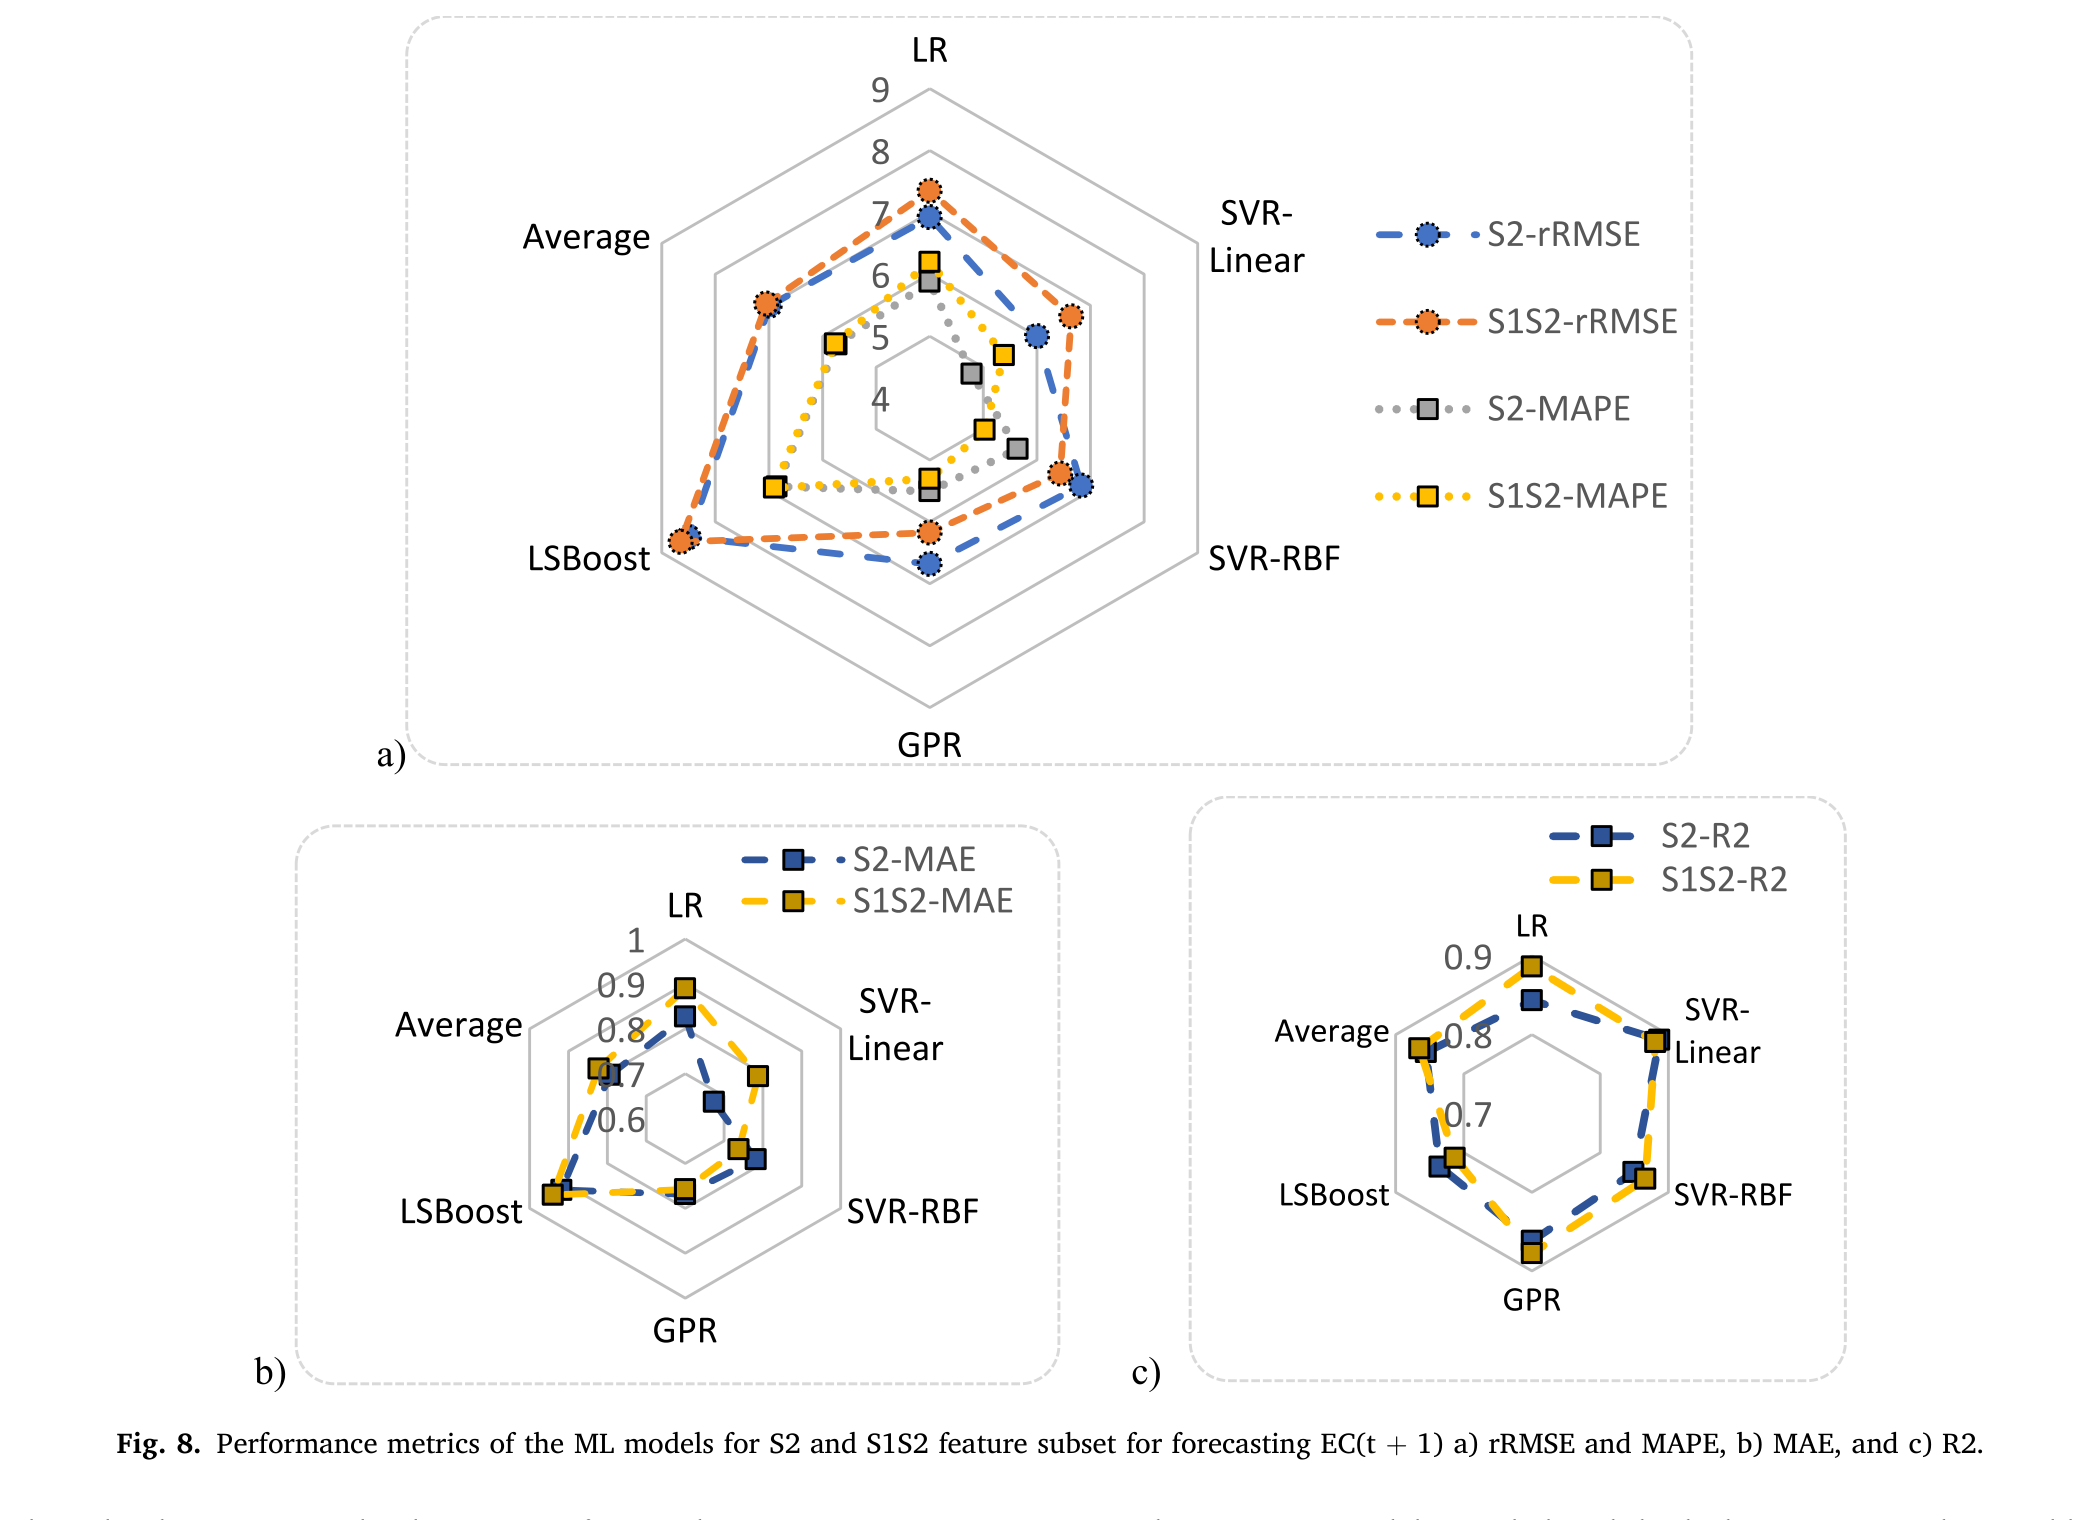
\includegraphics[width=0.98\textwidth,height=0.68\textheight,keepaspectratio]{figures/paper_original/fig08_model_metrics.png}
\caption{Hình 8 trong bài báo gốc: biểu đồ so sánh metric giữa S2 và S1S2. Nguồn: [1], tr. 15.}
\label{fig:orig-08}
\end{figure}

\begin{figure}[p]
\centering
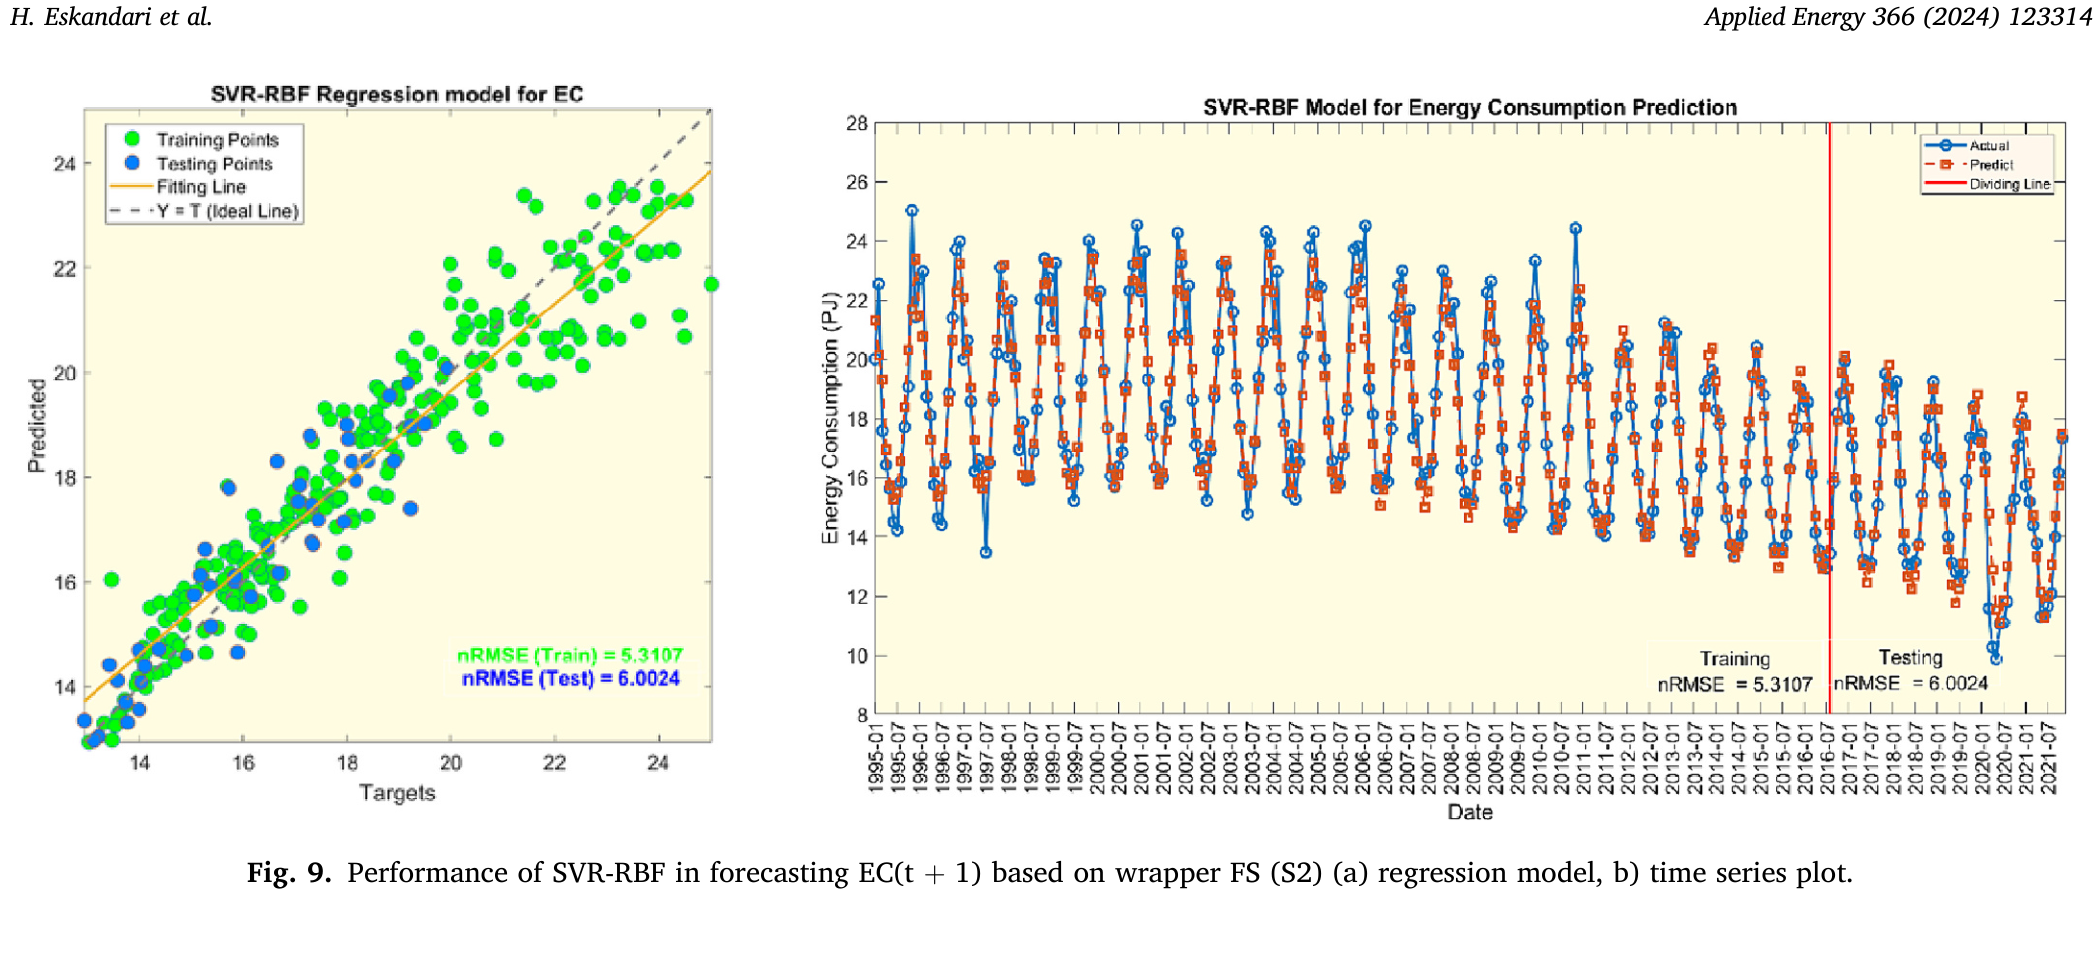
\includegraphics[width=0.98\textwidth,height=0.62\textheight,keepaspectratio]{figures/paper_original/fig09_s2_svr_rbf.png}
\caption{Hình 9 trong bài báo gốc: kết quả SVR-RBF với Wrapper S2, gồm regression plot và chuỗi dự báo. Nguồn: [1], tr. 16.}
\label{fig:orig-09}
\end{figure}

\begin{figure}[p]
\centering
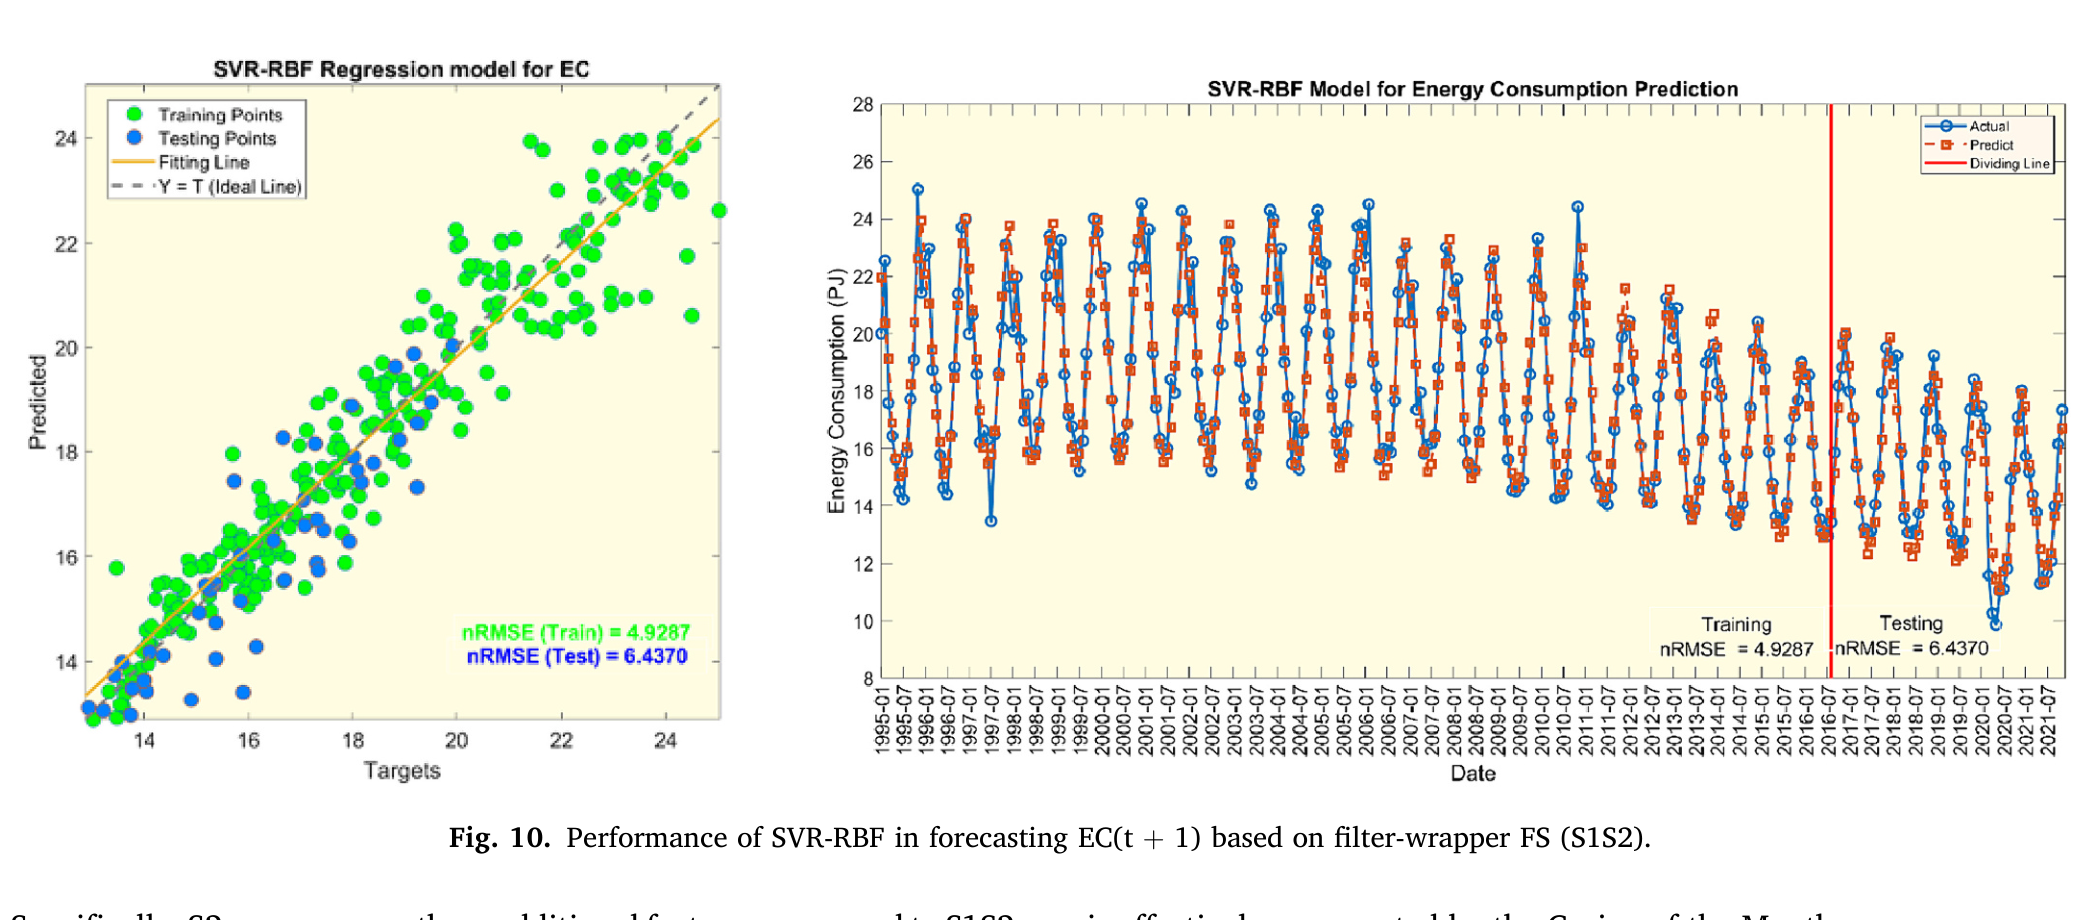
\includegraphics[width=0.98\textwidth,height=0.62\textheight,keepaspectratio]{figures/paper_original/fig10_s1s2_svr_rbf.png}
\caption{Hình 10 trong bài báo gốc: kết quả SVR-RBF với Ensemble Filter-Wrapper S1S2. Nguồn: [1], tr. 16.}
\label{fig:orig-10}
\end{figure}

\section{Các hình SHAP}

\begin{figure}[p]
\centering
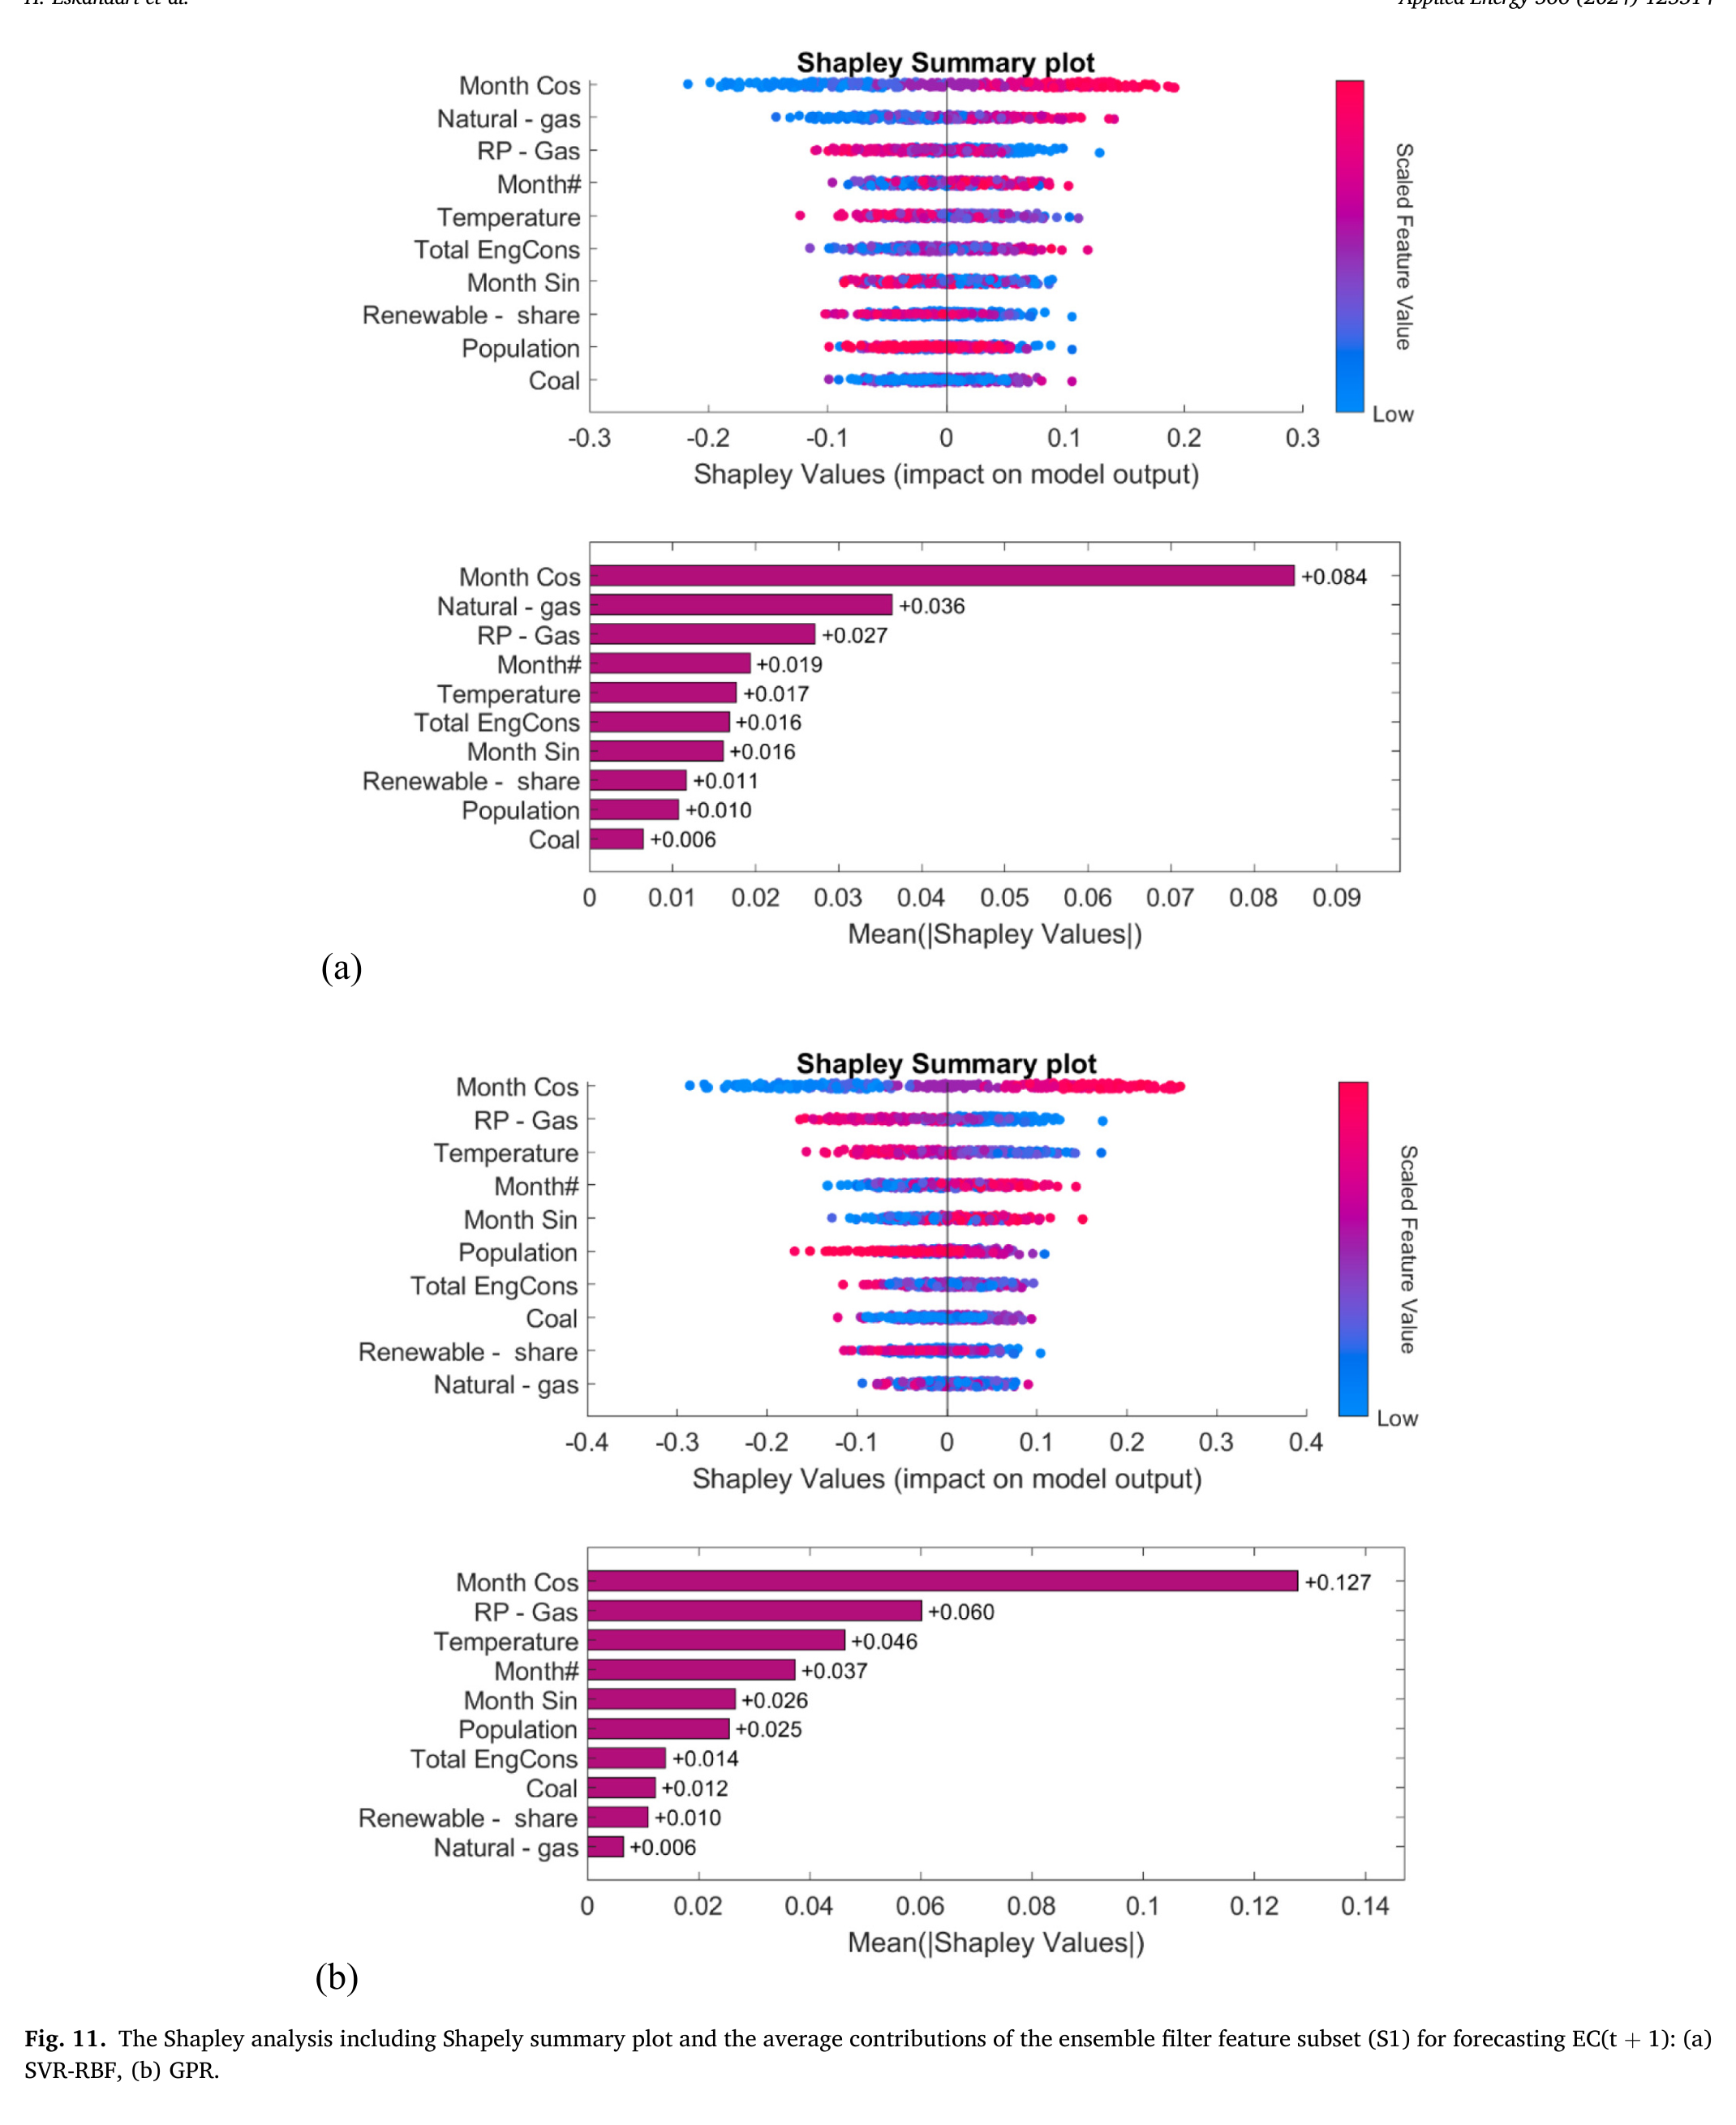
\includegraphics[width=0.88\textwidth,height=0.78\textheight,keepaspectratio]{figures/paper_original/fig11_shap_s1.png}
\caption{Hình 11 trong bài báo gốc: SHAP summary và Mean absolute SHAP của S1 với SVR-RBF và GPR. Nguồn: [1], tr. 17.}
\label{fig:orig-11}
\end{figure}

\begin{figure}[p]
\centering
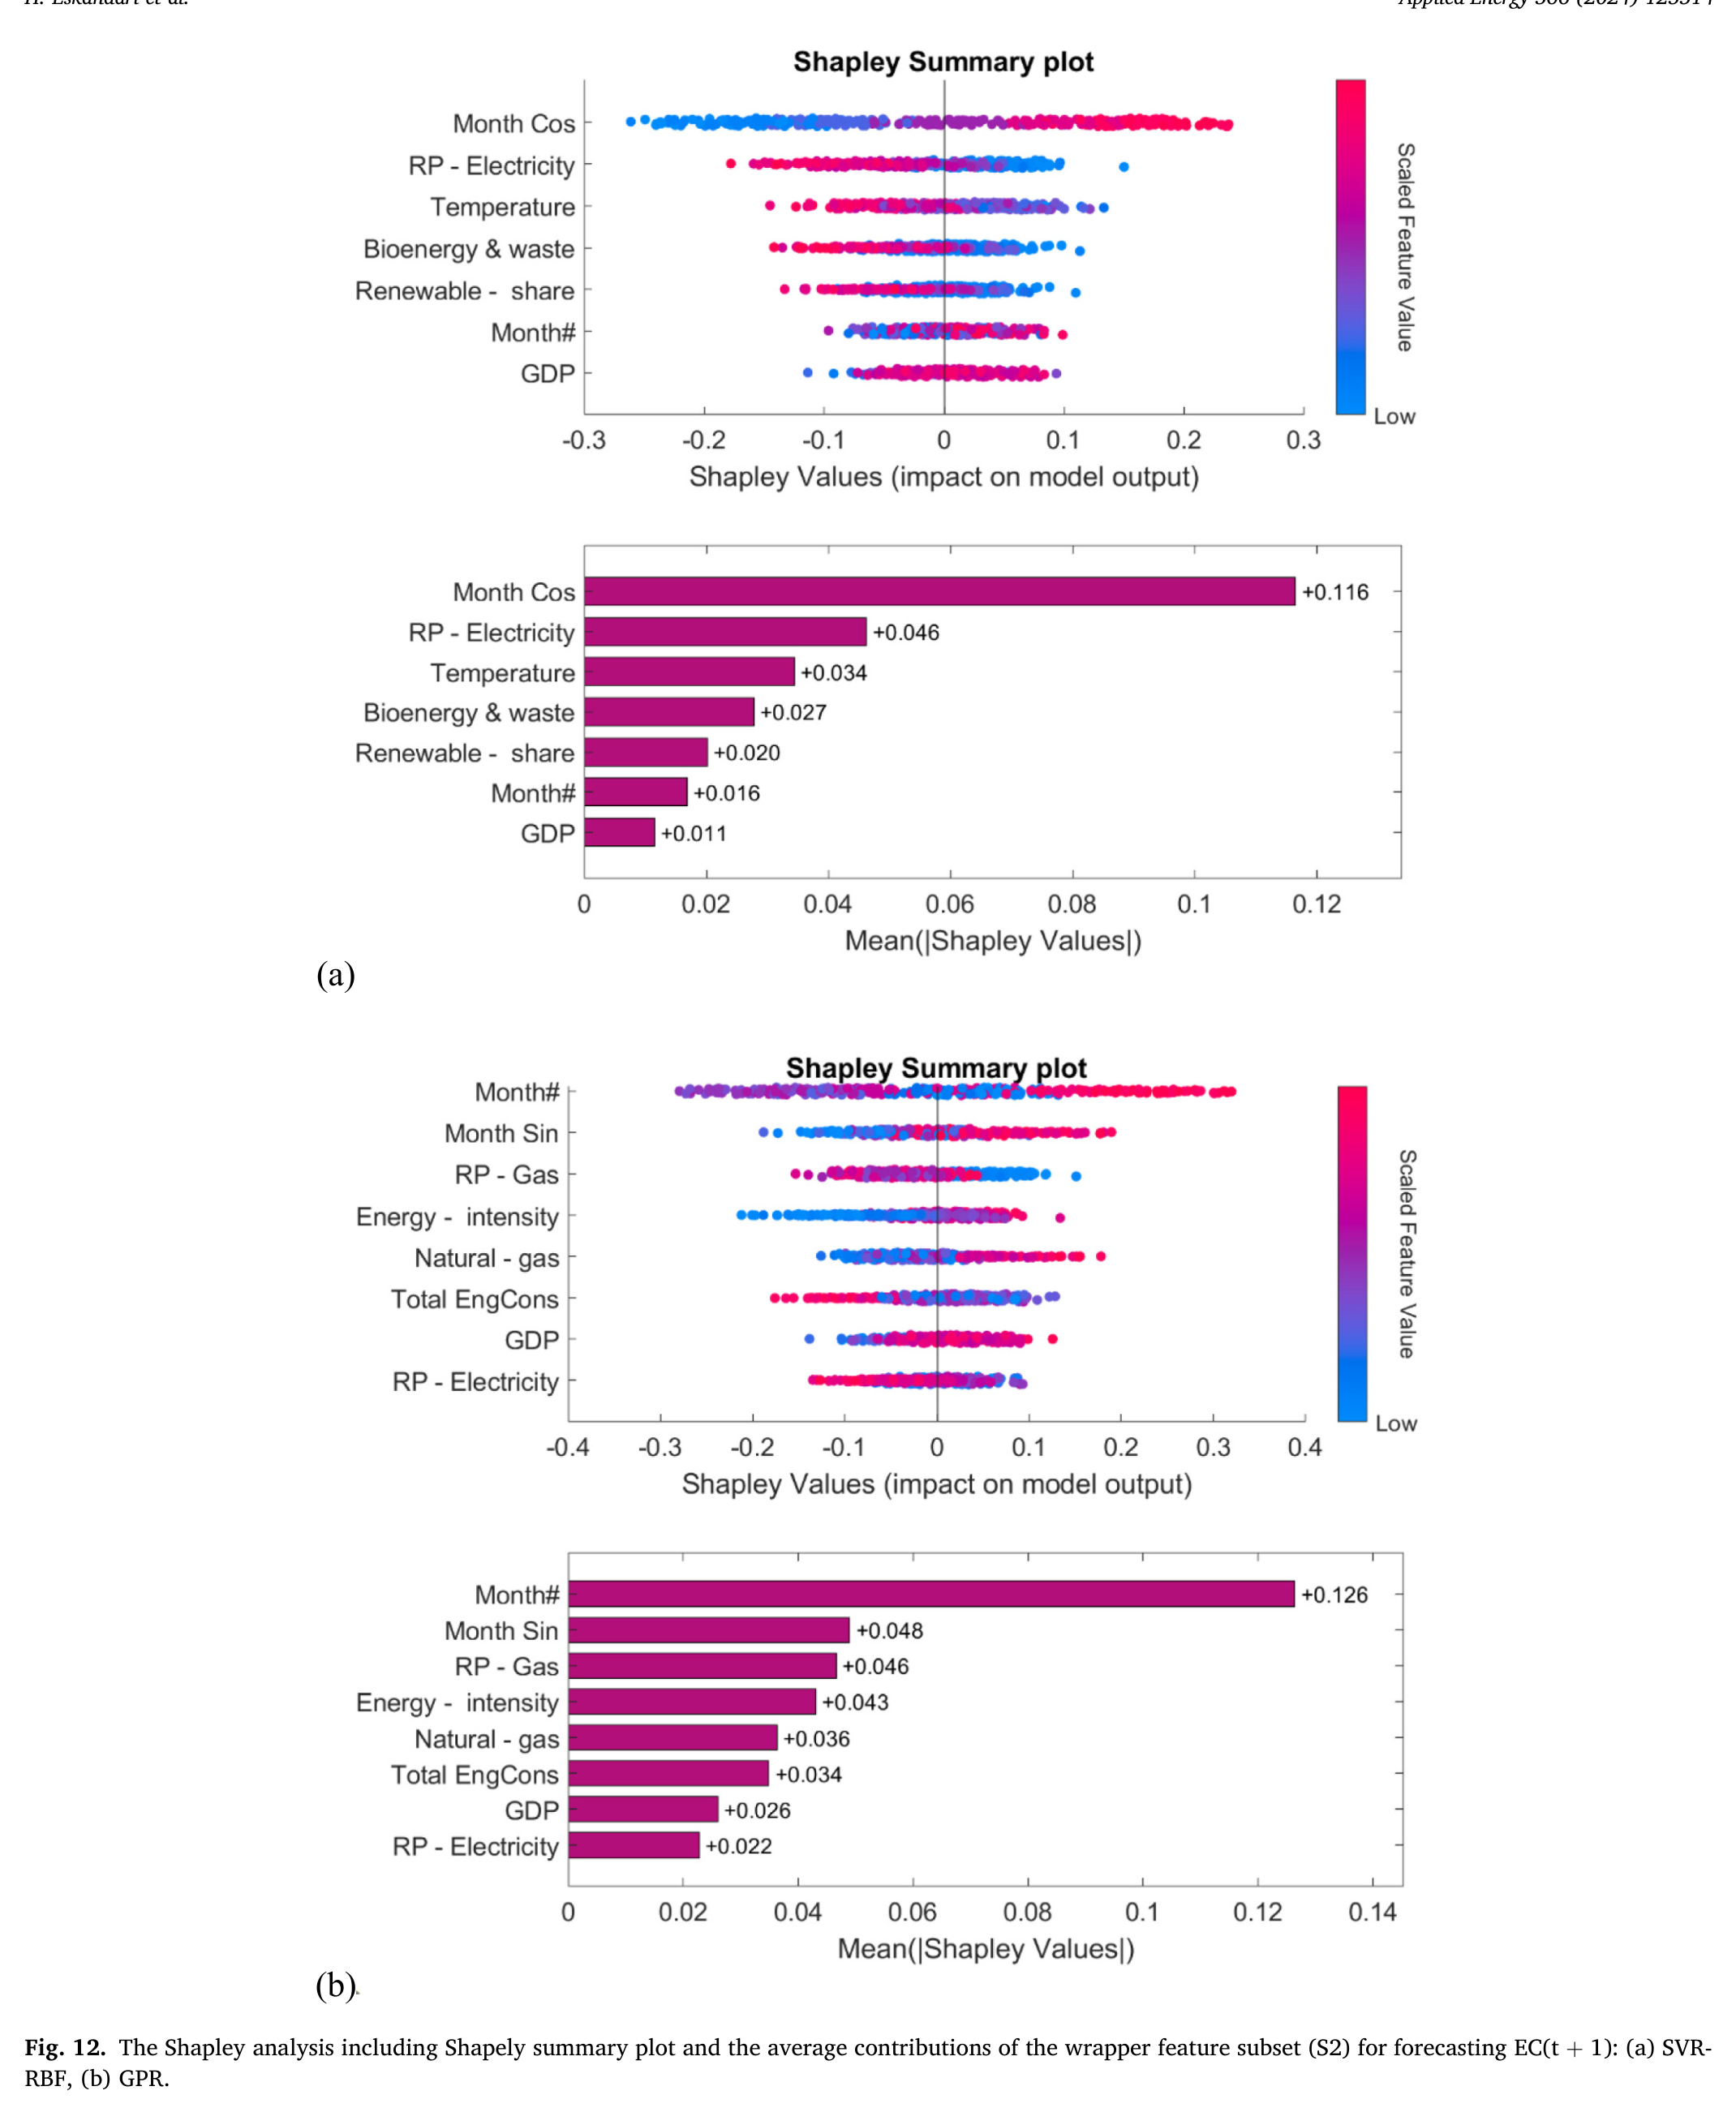
\includegraphics[width=0.88\textwidth,height=0.78\textheight,keepaspectratio]{figures/paper_original/fig12_shap_s2.png}
\caption{Hình 12 trong bài báo gốc: SHAP summary và Mean absolute SHAP của S2 với SVR-RBF và GPR. Nguồn: [1], tr. 18.}
\label{fig:orig-12}
\end{figure}

\begin{figure}[p]
\centering
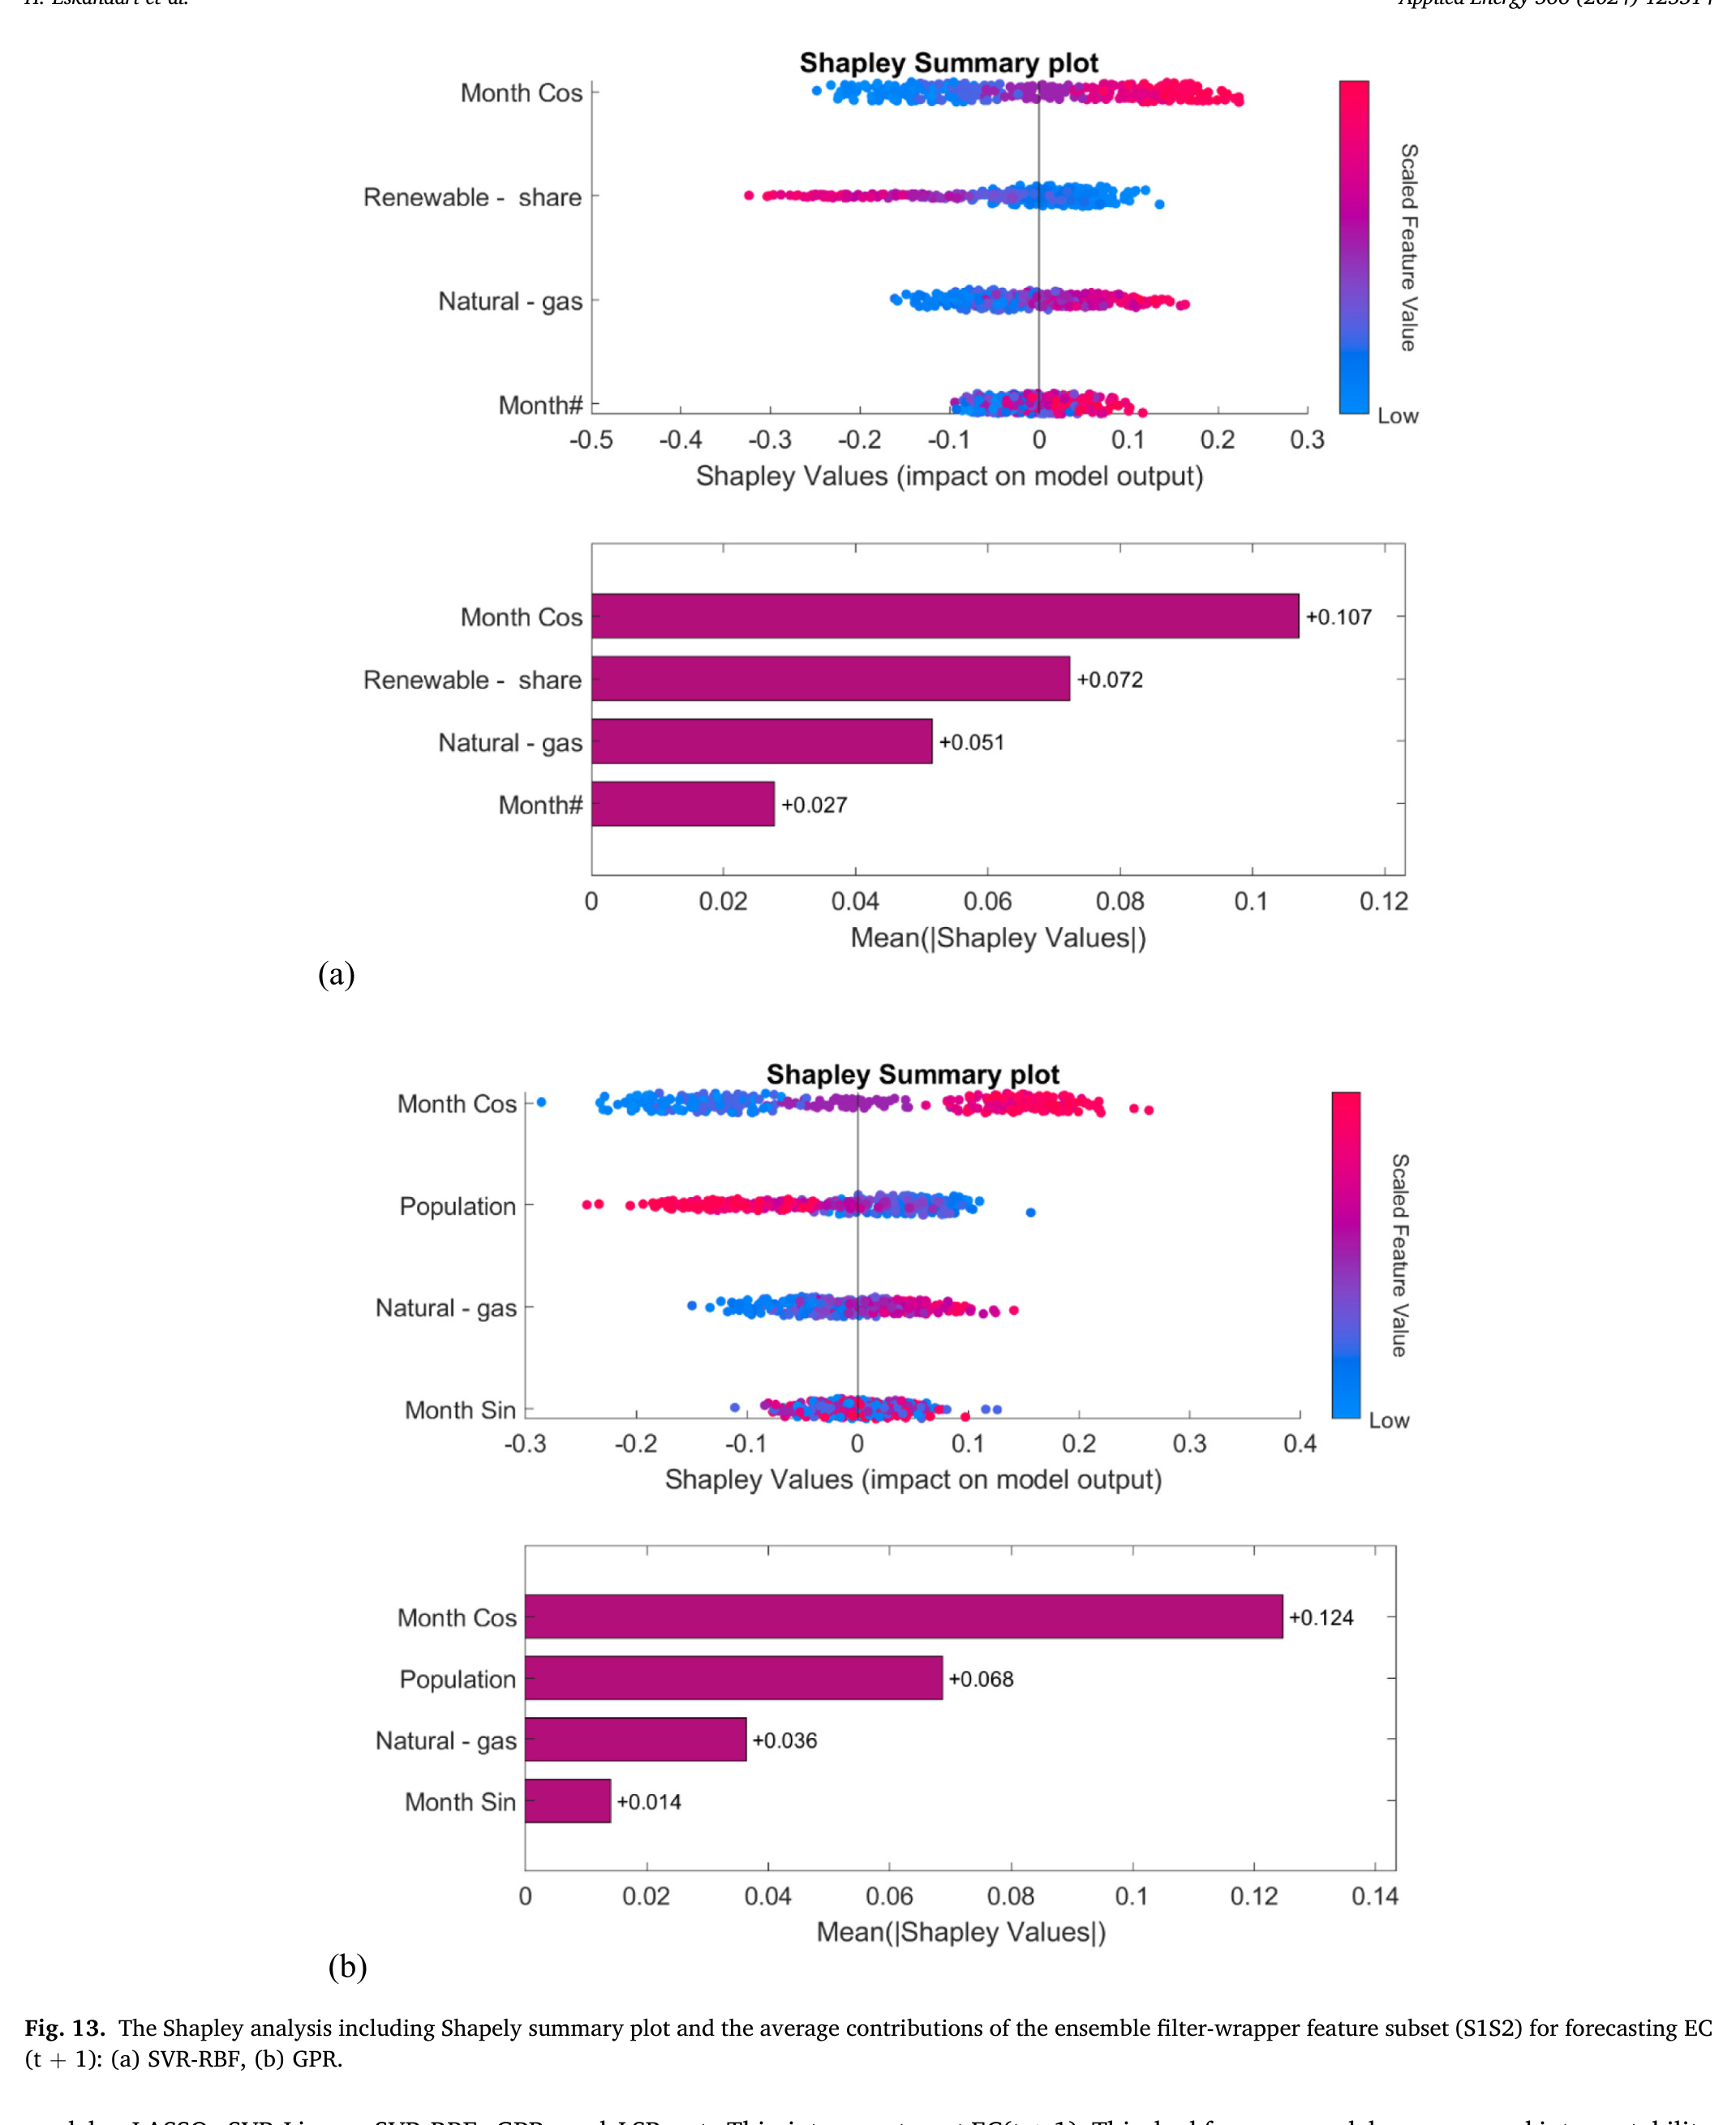
\includegraphics[width=0.88\textwidth,height=0.78\textheight,keepaspectratio]{figures/paper_original/fig13_shap_s1s2.png}
\caption{Hình 13 trong bài báo gốc: SHAP summary và Mean absolute SHAP của S1S2 với SVR-RBF và GPR. Nguồn: [1], tr. 19.}
\label{fig:orig-13}
\end{figure}

\section{Bản trích nguyên gốc các bảng Feature Selection và forecasting}

\begin{landscape}
\begin{table}[p]
\centering
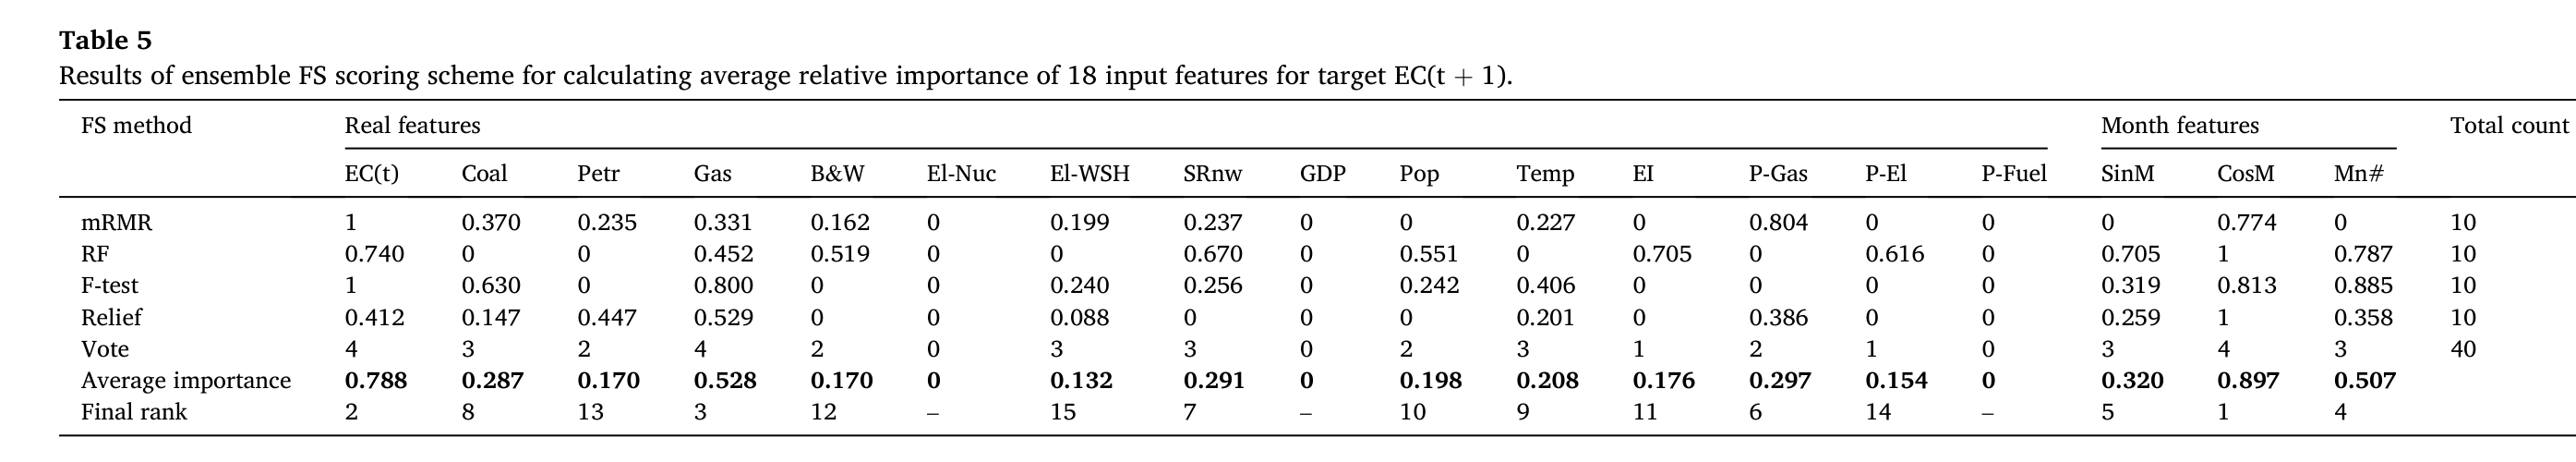
\includegraphics[width=0.96\linewidth,height=0.62\textheight,keepaspectratio]{figures/paper_original/table_5_original.png}
\caption{Bản trích nguyên gốc Table 5: điểm và thứ hạng Ensemble Filter cho 18 đặc trưng. Nguồn: [1], tr. 14.}
\label{tab:orig-5-image}
\end{table}
\end{landscape}

\begin{landscape}
\begin{table}[p]
\centering
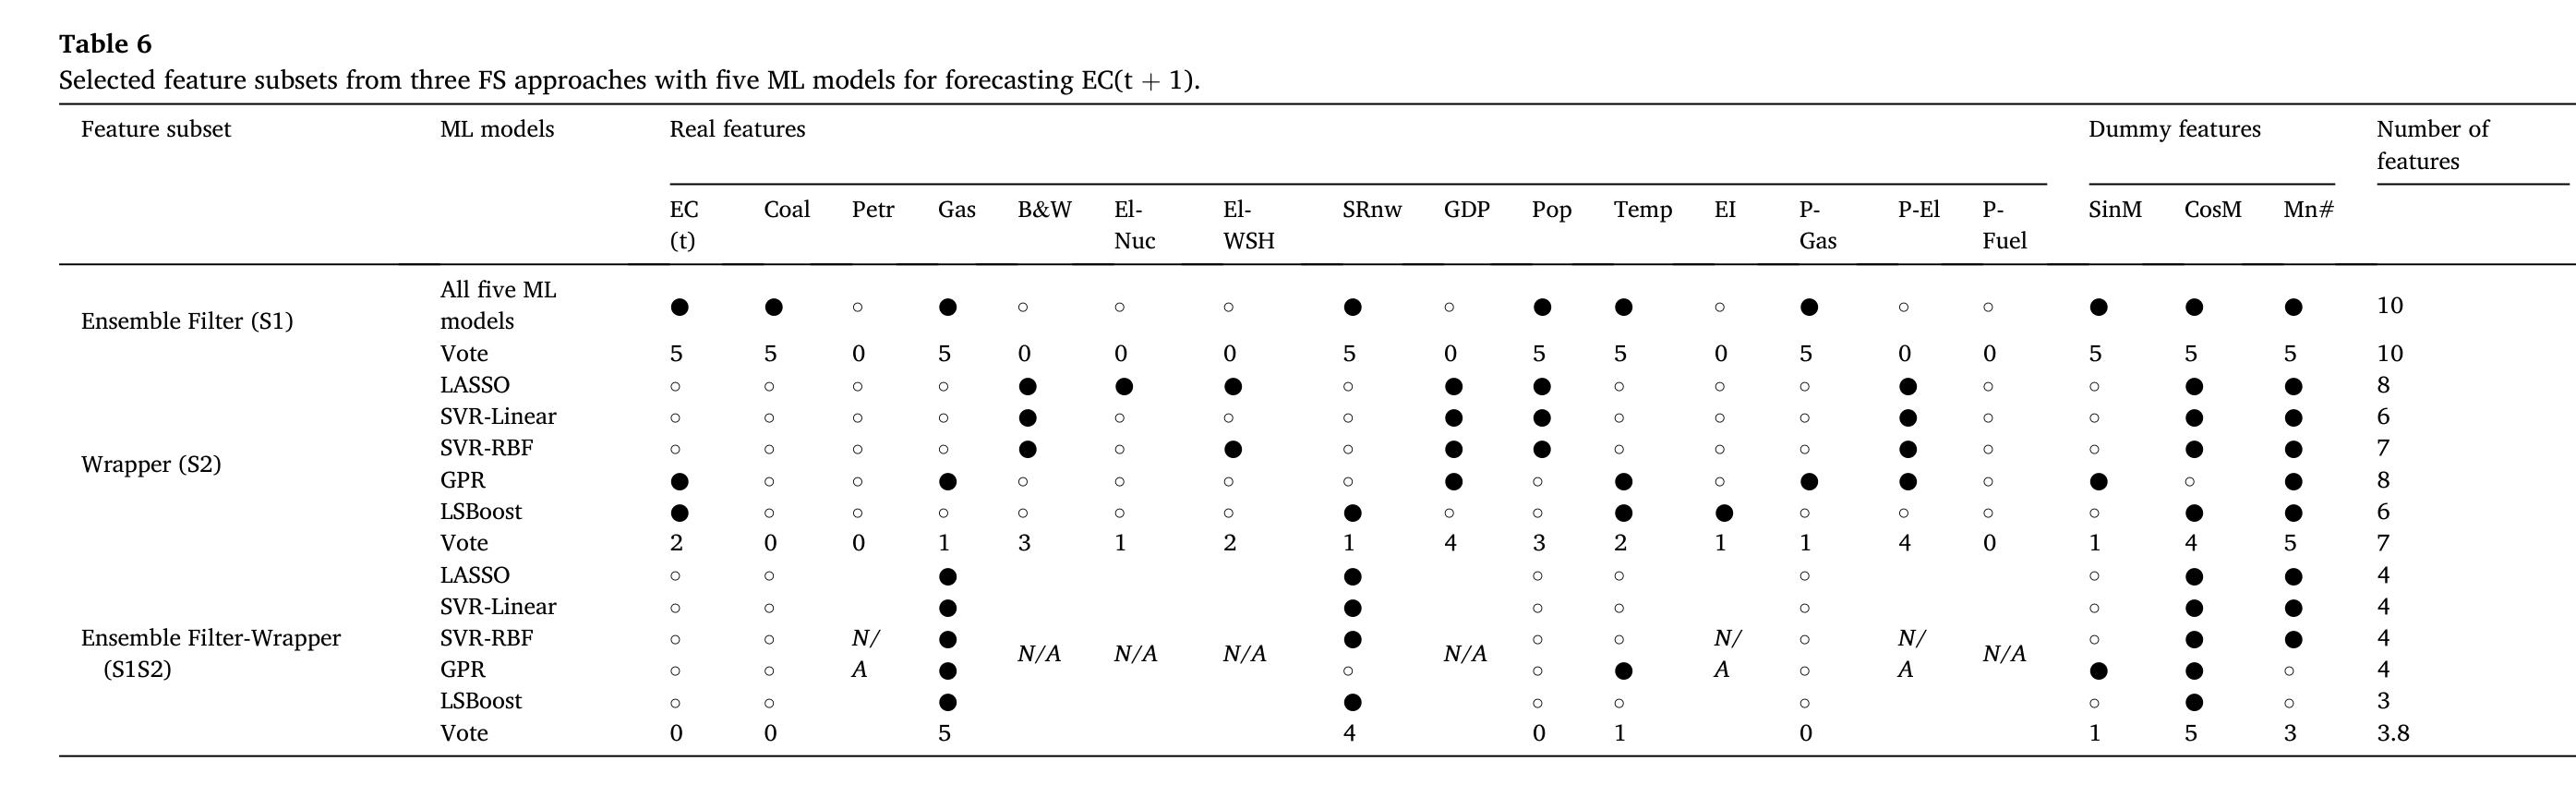
\includegraphics[width=0.96\linewidth,height=0.72\textheight,keepaspectratio]{figures/paper_original/table_6_original.png}
\caption{Bản trích nguyên gốc Table 6: các tập đặc trưng S1, S2 và S1S2 theo từng ML model. Nguồn: [1], tr. 14.}
\label{tab:orig-6-image}
\end{table}
\end{landscape}

\begin{landscape}
\begin{table}[p]
\centering
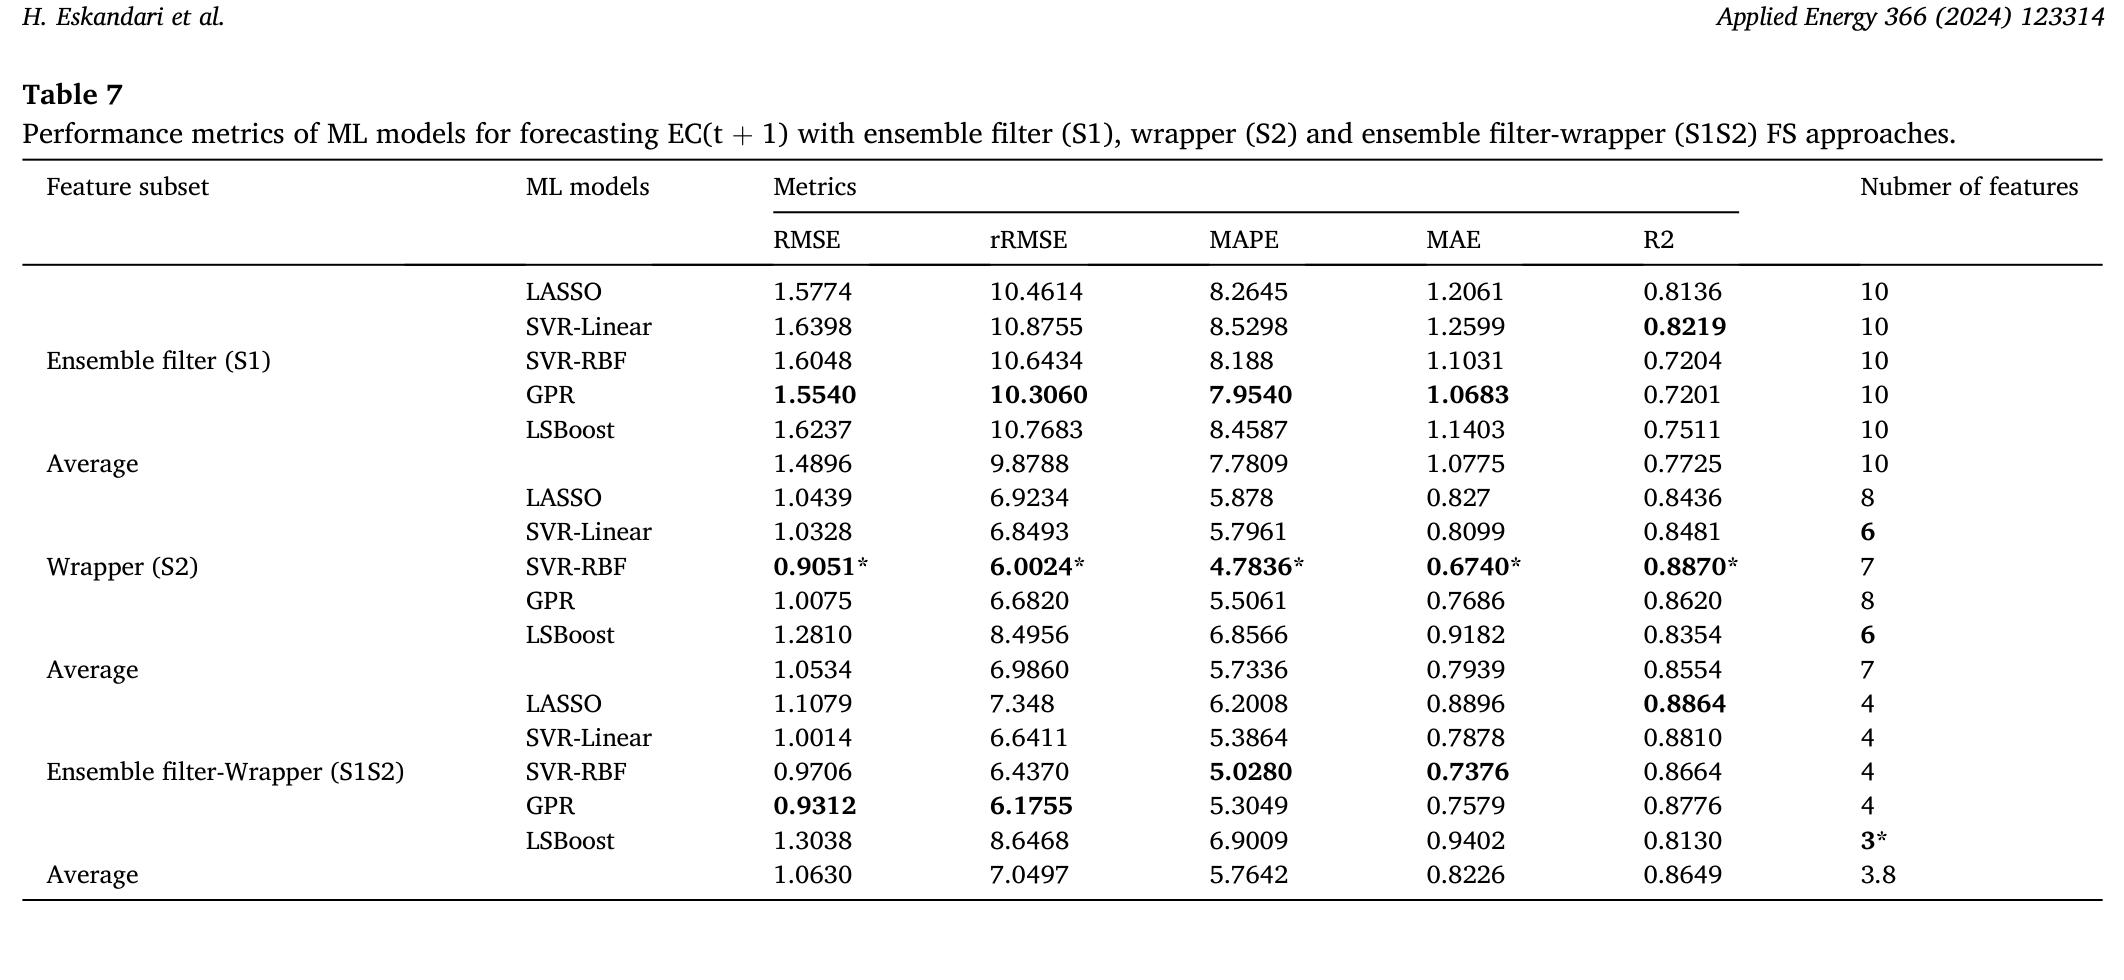
\includegraphics[width=0.96\linewidth,height=0.72\textheight,keepaspectratio]{figures/paper_original/table_7_original.png}
\caption{Bản trích nguyên gốc Table 7: các metric dự báo của 15 cấu hình S1, S2 và S1S2. Nguồn: [1], tr. 15.}
\label{tab:orig-7-image}
\end{table}
\end{landscape}

\noindent Các bảng số liệu có thể đọc và trích dẫn trong nội dung chính được trình bày lại dưới dạng bảng LaTeX tại Chương 5. Ảnh nguồn trong phụ lục được giữ để người đọc có thể kiểm tra cách trình bày ban đầu của tác giả.
